\chapterimage{sheaves.jpg}
\chapter{Sheaves}
\section{Motivating example}
\begin{exr}
Prove that $\scm_p:=$\{germs that vanishing at $p$\} is the only maximal ideal in $\calo_p$(Hint: prove that $\calo_p-\scm_p\subseteq \calo_p^{\times}$)
\end{exr}
\begin{proof}In general setting, consider a ring $A$.
The set of non-unit can be written as $\cup\scm_j$, where each $\scm_j$ is a maximal ideal in $A$. $A-\scm\subseteq A^\times\Lrta A-\scm\subseteq A-\cup_j\scm_j\Lrta \scm\supseteq\cup_j\scm_j$, then there is only one maximal ideal. It suffices to prove each element in $\calo_p-\scm_p$ is invertible. 

Use $(f,U)_p$ to denote the equivalent class of $(f,U)$.
$(f,U)_p\in \calo_p-\scm_p\Lrta f(p)\neq 0$, because $f$ is continuous on $U$, there exists an open set $V\subseteq U$, s.t. $f(q)\neq0,\forall q\in V\Lrta (1/f,V)$ is an inverse.
\end{proof}

\begin{exr}
Prove that $\frac{\scm_p}{\scm_p^2}\cong T^*_pX$, $T^*_p X$ is the cotangent bundle of differentiable manifold $X$ at $p$. 
\end{exr}
\begin{proof}Construct explicitly the isomorphism:
$$
(f,V)_p+\scm_p^2\longmapsto df_p=\sum_i\left.\frac{\partial f\circ \varphi^{-1}}{\partial x^i}\right|_p (dx^i)_p,
$$ 
where for a given tangent vector $\delta_p\in T_p X\cong Der_p(C^{1}(X))$ at $p$, $df_p(\delta_p)=\delta_p f\in \reals$ is an $\reals$-linear map. It is well-defined because $h\in \scm_p^2\Lrta d h_p=0$ and $(g,U)\sim (f,V)$, then there exists an open $p\in W\subseteq U\cap V$, s.t. $f|_W-g|_W=0$, $(df_p-dg_p)(\delta)=\delta_p(f)-\delta_p(g)$. Consider a bump function $\phi(x)=1,\forall x\in W'\ni p$ and $\phi(x)=0,\forall x\in U\cap V-W$, then $0=\delta_p(f|_{W'}-g|_{W'})=\delta_p((f-g)\phi|_{W'})=(f(p)-g(p))\delta_p(\phi)+\delta_p(f-g)\phi(p)\Lrta \delta_p(f-g)=0$.

It is surjective because the basis $(dx^j)_p$ can be generated by this map.

Construct the inverse map. Consider a chart of $p$, $(V,\varphi)$ s.t. $\varphi(p)=0\in \reals^n$, and define $x_i$ to be the $i$-th entry of $\phi$
$$
\sum_i a_i (dx^i)_p\longmapsto \left(\sum_i a_i x_i, V \right)+\scm^2_p.
$$
To check this is indeed a inverse, we only need to check (The other direction is tricial)
$$
(f,V)_p+\scm_p^2=\left(\sum_i\left.\frac{\partial f\circ \varphi^{-1}}{\partial x^i}\right|_0 x^i, V'\right)+\scm_p^2.
$$
But, assuming $\varphi(V)$ to be a star-shaped domain in $\reals^n$: 
$$
f\circ\varphi^{-1}(x)= \left(\int_0^1d t\frac{\partial f\circ\varphi^{-1}(t x)}{\partial t}\right)=\sum_ix^i\underbrace{\int_0^1d t\frac{\partial f\circ\varphi^{-1}}{\partial x^i}(t x)}_{:=h_i(x)}.
$$
Though $h_i(x)$ is at most continuous, $\sum_i x^i h_i(x)$ is differentiable and $$
h_i(0)=\left.\frac{\partial f\circ \varphi^{-1}}{\partial x^i}\right|_0
\Lrta h_i(x)-\left.\frac{\partial f\circ \varphi^{-1}}{\partial x^i}\right|_0\in \scm_p
$$
then
$$
\sum_i x^i \left(h_i(x)-\left.\frac{\partial f\circ \varphi^{-1}}{\partial x^i}\right|_0\right)\in \scm_p^2
$$
\end{proof}
\section{Definition of presheaf and sheaf}
\begin{exr}
Verify that the data of a presheaf is precisely the data of a contravariant functor from the category of open sets of $X$ to the category of sets.
\end{exr}
\begin{proof}We use a diagram to replace all the words:
\begin{center}
\begin{tikzcd}
U\ar[loop left] \arrow[d, "\calf"] \arrow[r, hook] & V \arrow[d, "\calf"] \arrow[r, hook] & W \arrow[d, "\calf"] \\
\calf(U)\ar[loop left, "res_{U,U}"] & \calf(V) \arrow[l, "{res_{V,U}}"'] & \calf(W) \arrow[l, "{res_{W,V}}"'] \arrow[ll, "{res_{W,V}}", bend left]
\end{tikzcd}
\end{center}
\end{proof}

\begin{exr}
Show that the following are presheaves on $\cplx$ (with the classical topology), but not sheaves: (a) bounded functions, (b) holomorphic functions admitting a holomorphic square root.
\end{exr}
\begin{proof}
\begin{enumerate}[label=(\alph*)]
\item Bounded functions $B$ is a presheaf, with the restriction map just the ordinary restriction of functions. But $B$ is not a sheaf because there could be an open cover $\{U_i\}_{i\in I}$(necessarily infinite), for example $U_n:=\{z\in\cplx: n-1< \text{Re}z<n+1\}$, and we can choose $f_n(z):=z$. each is bounded function on the open set, but there is no global bounded function that restricts to them.
\item Holomorphic functions admitting a square roots, in other words, they are of the form $h^2(z)$ where $h(z)$ is a holomorphic function. It is a presheaf with ordinary restrictions and it is not a sheaf because it violate the gluability axiom. Consider $U$ to  be a strip $\{2<|z|<3 \}$ and $U$ is covered by open disks $D_n:=\{|z-5/2e^{i n2\pi/10}|<1\}$, on each open disk, there is a holomorphic square root corresponding to $\sqrt z$. But there is no $\sqrt z$ defined on the strip $U$.
\end{enumerate}
\end{proof}
\begin{exr}
The identity and gluability axioms may be interpreted as saying that $\calf(\cup_{i\in I}U_i)$ is a certain limit. What is that limit?
\end{exr}
\begin{proof}
The index category $\cali$ is the ``subsets index by $I$'' with inclusion being the morphism it is a partially ordered set. Or we can simply denote it by $I$ with $i\leq j$ iff $U_i\inj U_j$. Then $\calf(\cup_{i\in I}U_i)$ can be interpreted as a limit with morphism $\calf(\cup_{i\in I}U_i)\lrta \calf(U_k)$ being the restriction $\res_{\cup_i U_i, U_k}$
$$
\calf(\cup_{i\in I}U_i)=\invlim_{i\in I}\calf(U_i)
$$
\end{proof}
\begin{exr}\ 
\begin{enumerate}[label=(\alph*)]
\item
 Verify that the the following examples are indeed sheaves ( differentiable functions, or continuous functions, or smooth functions, or functions on a manifold or $\reals^n$).
 \item  Show that real-valued continuous functions on (open sets of) a topological space X form a sheaf.
\end{enumerate}
\end{exr}
\begin{proof}
\begin{enumerate}[label=(\alph*)]
\item All of them are easily seen to be presheaves, we only need to verify they satisfies the identity axiom and gluability axiom of sheaf.

Identity axiom holds for all of them, $\res_{U,U_i}f_1=\res_{U,U_i}f_2,\forall U_i$ means $f_1(p)=f_2(p)\forall p\in U_i,\forall U_i$. Hence $f_1$ and $f_2$ coincide on each point in $U$, they are equal. (This is not true for functions on schemes)

Manifolds are Hausdorff and paracompact, hence endowed with partition of unity. For each over cover $\{U_i\}_{i\in I}$, there is a partition of unity $\{\rho_i\}_{i\in I}$ subordinate to it (each $\rho_i$ is non-negative and continuous, and we can choose it to be smooth if the manifold is smooth). For $\{f_i\in C^{k}(M)\}$ compatible on the intersections, we can define $f=\sum_i \rho_i(x)f_i(x)\in C^{k}(M)$. Such that it restrict to each $f_i$. $C^k(M)$ can be continuous, smooth, or even just plain functions.
(In particular the partition of unity property is included in the notion of fine sheaves. In fact, we don't need partition of unity to prove $(a)$ here.)

\item Continuous functions on a topological space $C(X)$. It is a presheaf. We don't have to worry about the fact that function may be not determined by it's value at points, because here the continuous function means continuous map from $X$ to $\reals$ and is indeed determined valuewise. 

For identity axiom, $f_1(p)=f_2(p)$ at every point in $U$. Then they are equal. 

For gluability axiom, we define $f(p)=f_i(p)$, where $f_i\in C(U_i)$ and $p\in U_i$. Then it remains to prove $f$ is a continuous function on $U$. Recall the definition of continuous function in terms of neighborhoods. Consider $f(p)\in \reals$, for any neighborhood $V$ of $f(p)=f_i(p)$. Because $f_i$ is continuous, there is a neighborhood $p\in W\subset U_i$ such that $f_i(W)\subset V$. $W$ is also an open subset in $U$. $\res_{U,W}f=\res_{U_s,W}\circ \res_{U,U_i}f=\res_{U_i,W}f_i$, hence $f(W)\subset V$. This means $f$ is continuous at every point $p$.
\end{enumerate}
\end{proof}

\begin{exr}
Now let $\calf(U)$ be the maps to $S$ that are locally constant, i.e., for any point $p$ in U, there is an open neighborhood of $p$ where the function is constant. Show that this is a sheaf. (A better description is this: endow $S$ with the discrete topology, and let $\calf (U)$ be the continuous maps $U \lrta S$.) This is called the constant sheaf (associated to $S$); do not confuse it with the constant presheaf. We denote this sheaf $\underline{S}$.
\end{exr}
\begin{proof}
The restriction maps are just the ordinary restrictions. The constant sheaf is indeed a sheaf because it is continuous functions from $U$ to $S$ where $S$ is with discrete topology. The proof is identical. Ae will be explained in the next exercise, in fact by \href{https://en.wikipedia.org/wiki/Pasting_lemma}{pasting lemma}, every presheaf of continuous maps $C(X,Y)$ is in  fact a sheaf. 
\end{proof}

\begin{exr}\label{chap2exr:sheaf_of_continuous_maps}
Suppose $Y$ is a topological space. Show that ``continuous maps to $Y$'' form a sheaf of sets on $X$. More precisely, to each open set $U$ of $X$, we associate the set of continuous maps of $U$ to $Y$. Show that this forms a sheaf.
\end{exr}
\begin{proof}
It is obviously a presheaf and the identity holds true.

As for the gluability. Choose $V$ an open set in $Y$, and the preimage of $f\in C(X,Y)$ defined point wise by $f_i\in C(U_i,Y)$, where $U_i$ is in the subset topology.
$$
f^{-1}(V)=\cup_i f_i^{-1}(V).
$$
Each $f_i^{-1}(V)$ is open set in $U_i$ hence is an open set in $X$.
\end{proof}

\begin{exr}\ 
\begin{enumerate}[label=(\alph*)]
\item 
(sheaf of sections of a map) Suppose we are given a continuous map $\mu : Y \lrta X$. Show that sections of $\mu$ form a sheaf. More precisely, to each open set $U$ of $X$, associate the set of continuous maps $s: U \lrta  Y$ such that $\mu\circ s   = id|_U$. Show that this forms a sheaf. 
\item Suppose that $Y$ is a topological group. Show that continuous maps to $Y$ form a sheaf of groups.
\end{enumerate}
\end{exr}
\begin{proof}\ 
\begin{enumerate}[label=(\alph*)]
\item It is a presheaf, and with obvious restriction maps. $s_i:=\res_{U,U_i}s$ and $\mu\circ s_i=id_{U_i}$. 

Given an open cover $\{U_i\}_{i\in I}$ of $U$.

Identity Axiom:  if $s_1,s_2$ agree when restricted to any $U_i$, then they agree point wisely.

Gluability Axiom: if $\{s_i\}_{i\in I}$  are compatible on each intersection. We define $s$ point wisely, we have to check $\mu\circ s=id|_U$. And this can be checked also value-wisely.
\item A topological group is a topological space together with  compatible group structures.

It is presheaf of groups, $s_1,s_2:U\lrta Y$ the multiplication is defined as $s_1 \cdot s_2(p)=s_1(p)\times s_2(p)$. The identity and inverse is also defined point-wisely. 

Given an open cover $\{U_i\}_{i\in I}$.

Identity axiom: if $s_1,s_2$ agree upon restricted to each $U_i$, then they agrees pint-wisely.

Gluability axiom: if $\{s_i\}_{i\in I}$  are compatible on each intersection. We define $s$ point wisely, we have to check $s$ is indeed continuous, and this has been checked in Exercise~\ref{chap2exr:sheaf_of_continuous_maps}.

 In fact, the group structure has nothing to do with whether it is a sheaf of sets.
 What we have to do is just to verify that the sheaf of sets possesses the addition structure of sheaf of groups.
\end{enumerate}
\end{proof}

\begin{exr}
 THE PUSHFORWARD SHEAF OR DIRECT IMAGE SHEAF. Suppose $\pi: X \lrta Y$ is a continuous map, and $\calf$ is a presheaf on $X$. Then define $\pi_*\calf$ by $\pi_*\calf(V)=\calf(\pi^{-1}(V))$, where $V $ is an open subset of $Y$. Show that $\pi_*\calf$ is a presheaf on $Y$, and is a sheaf if $\calf{F}$ is. This is called the \textbf{pushforward} or \textbf{direct image} of $\calf$. More precisely, $\pi_*\calf$ is called the pushforward of $\calf$ by $\pi$.
\end{exr}
\begin{proof}
It is a presheaf:
The new restriction map is induced as 
$$
\res'_{V,W}=\res_{\pi^{-1}V,\pi^{-1}W}.
$$
The functorial property holds
$$
\res'_{V,V}=\res_{\pi^{-1}V,\pi^{-1}V}=id_{\calf(\pi^{-1}(V))}:=id_{\pi_*\calf(V)}
$$
and
$$
\res'_{U,V}\circ \res'_{V,W}=\res_{\pi^{-1}U,\pi^{-1}V}\circ \res_{\pi^{-1}V,\pi^{-1}W}=\res_{\pi^{-1}U,\pi^{-1}W}=\res'_{V,W}.
$$

Now assume $\calf$ is a sheaf.
The open cover $\{V_i\}_{i\in I}$ of $V$ pullback to an open cover $\pi^{-1}(V_i)$ of $\pi^{-1}(V)$.

Identity axiom: $f_1,f_2$ in $\pi_*\calf(V)$ agrees when restricted to any $V_i$, then $f_1,f_2$ as element in $\calf(\pi^{-1}{V})$ agrees when restricted to each $\pi^{-1}(V_i)$. Because $\calf$ is a sheaf, $f_1,f_2$ has to agree in $\calf(\pi^{-1}(V))$, which is equivalent to $f_1,f_2$ agrees in $\pi_*\calf(V)$.

Gluability axiom: if $\{f_i\}_{i\in I}$  are compatible on each intersection. They are also compatible as sections in $\calf(\pi^{-1}V_i)$, because $\calf$ is a sheaf, there is an element $\tilde{f}\in \calf(\pi^{-1}V)$ such that it restricts to each $f_i$. $\tilde{f}$ can be interpreted as an element $f\in \pi_*\calf(V)$.
\end{proof}

\begin{exr}\label{chap2exr:Pushforward_induces_morphism_stalks}
Suppose $\pi: X \lrta Y $ is a continuous map, and $\calf$ is a sheaf of sets (or rings or $A$-modules) on $X$. If $ \pi(p) = q$, describe the natural morphism of stalks $(\pi_*\calf)_q \lrta \calf_p$.
\end{exr}
\begin{proof}
First we define the morphism of stalk using the universal property of colimits.
$$
\calf_p=\dirlim\calf(U),
$$
 where the index category is the ``open sets that containing $p$'' and each $\pi_*\calf(V)\cong \calf(\pi^{-1}(V))$
\begin{center}
\begin{tikzcd}
\pi_*\calf_q \arrow[rr, "\exists!", dashed] &  & \calf_p \\
 & \calf(\pi^{-1}V_i) \arrow[ru, "g_i"] \arrow[r] & \calf(\pi^{-1}V_j) \arrow[u, "g_j"] \\
\pi_*\calf(V_i) \arrow[r] \arrow[uu, "f_i"] \arrow[ru, "="] & \pi_*\calf(V_j) \arrow[luu, "f_j"'] \arrow[ru, "="] &
\end{tikzcd}
\end{center}
Because the index category of either colimits is filtered set. We can equivalently define the at the level of disjoint union modulo equivalence. 
$$
\calf_p:=\left\{(f_i; U_i)\in\coprod_{i\in\cali} \calf(U_i):\right\}\left/
\left(
\begin{matrix}
& (f_i;U_i)\sim (f_j;U_j)\text{iff there are $\res_{U_i\rta U_k}:\calf(U_i)\rta \calf(U_k)$}\\
&\text{$\res_{U_j,U_k}:\calf(U_j)\rta \calf(U_k)$ s.t., $f_i|_{U_k}=f_j|_{U_k}\in \calf(U_k)$}
\end{matrix}
\right)
\right.
$$
$$
[(f_i;V_i)]\mapsto [(f_i;\pi^{-1}(V_i))]
$$
It is well defined map because
$$
\res'_{V,W}=\res_{\pi^{-1}V,\pi^{-1}W}.
$$
\end{proof}

\begin{definition}
Ringed spaces, and $\calo_X$-modules. Suppose $\calo_X$ is a sheaf of rings on a topological space $X$. Then $(X,\calo_X)$ is called a \textbf{ringed space}. The sheaf of rings is often denoted by $\calo_X$. This sheaf is called the structure sheaf of the ringed space. Sections of the structure sheaf $\calo_X$ over an open subset $U$ are called \textbf{functions} on $U$. Functions in this sense is not defined point wise, and is not determined by their value at points.
\end{definition}

\begin{exr}
If $(X,\calo_X)$ is a ringed space, and $\calf$ is an $\calo_X$-module, describe how for each $p\in X$, $\calf_p$ is an $\calo_{X,p}$-module.
\end{exr}
\begin{proof} The crucial print is that colimit of product is product of colimit.
\begin{center}
\begin{tikzcd}
 & \calo_X(V)\times \calf(V) \arrow[rr, "\text{action}"] \arrow[ld, "{\res_{V,U}\times\res_{V,U}}"'] \arrow[rdd] &  & \calf(V) \arrow[ld, "{\res_{V,U}}"] \arrow[rdd] &  \\
\calo_X(U)\times \calf(U) \arrow[rr, "\text{action}"] \arrow[rrd] &  & \calf(U) \arrow[rrd] &  &  \\
 &  & \calo_{X,p}\times\calf_p \arrow[rr, "\text{action}"] &  & \calf_p
\end{tikzcd}
\end{center}
At the explicit level,
$$
\calo_{X,p}\times \calf_p\ni([(a_V;V)],[(m_U;U)])=[((a_{W}, m_W);W)]\in (\calo_X\times \calf)_p,
$$
where $W\subset V\cap U$.
and 
$$
\calo_{X,p}\times \calf_p\ni([(a_V;V)],[(m_U;U)])\overset{\text{action}}{\longmapsto}[(a_w\cdot m_W;W)]\in\calf_p.
$$
And it is routine to verify that map defined above indeed gives $\calf_p$ the structure of a $\calo_p$ module.


\end{proof}
\section{Morphism of presheaves and sheaves}
\begin{exr}\label{chap2exr:morphism_of_sheaves_induce_on_stalks}
MORPHISMS OF (PRE)SHEAVES INDUCE MORPHISMS OF STALKS. If $\phi: \calf\lrta \calg $ is a morphism of presheaves on $X$, and $p \in X$, describe an induced morphism of stalks $\phi_p : \calf_p \lrta \calg_p$. Translation: taking the stalk at $p$ induces a functor $Sets_X \lrta  Sets$.
\end{exr}
\begin{proof}
Using the language of colimits,
\begin{center}
\begin{tikzcd}
\calf_q \arrow[rr, "\exists!\phi_p", dashed] &  & \calg_p \\
 & \calg(V_i) \arrow[ru, "g_i"] \arrow[r,"\res_{V_i,V_j}"] & \calg(V_j) \arrow[u, "g_j"] \\
\calf(V_i) \arrow[r,"\res_{V_i,V_j}"] \arrow[uu, "f_i"] \arrow[ru, "\phi(V_i)"] & \calf(V_j) \arrow[luu, "f_j"'] \arrow[ru, "\phi(V_j)"] &
\end{tikzcd}
\end{center}

Using the explicit construction, we can check the map 
$$
\phi_p:[(s;V)]\mapsto [(\phi(V)s;V)]
$$
is well-defined. Assume $(s;V)\sim (s';V')$, there exists $(t;W)$ so that $W\subset V\cap V'\ni p$ and $t=s|_W=s'|_W$.
 We can check $(\res_{V,W}\phi(V)s;W)=(\res_{V'W}\phi(V')s';W)=(\phi(W)t;W)$. Hence $[(\phi(V)s;V)]=[\phi(V')s';V']$.
\end{proof}

\begin{exr}
Suppose $\pi:X\lrta Y$ is a continuous map of topological spaces (i.e., a morphism in the category of topological spaces). Show that pushforward gives a functor $\pi_* : Sets_X \lrta Sets_Y$ . Here $Sets $ can be replaced by other categories. 
\end{exr}
\begin{proof}
We want ot verufy the diagram 
\begin{center}
\begin{tikzcd}
\calf \arrow[r, "\phi",blue] \arrow[d, "\pi_*"',red] & \calg \arrow[d, "\pi_*",red] \\
\pi_*\calf \arrow[r, "\pi_*(\phi)",blue] & \pi_*\calg,
\end{tikzcd}
\end{center}
where $\phi:\calf\lrta \calg$ is a morphism of sheaves and $\pi_*\phi(V)=\phi(\pi^{-1}V)$. 
In detail, it means each square is commutative in the following diagram
\begin{center}
\begin{tikzcd}
 &  & \calf(\pi^{-1}U) \arrow[lld,"\pi_*",red] \arrow[dd, bend left,"\phi", blue] &  \\
\pi_*\calf (U) \arrow[dd, bend right,"\pi_*(\phi)"', blue] &  & \pi^{-1}U \arrow[u] \arrow[rd, hook] \arrow[d] & \calf(\pi^{-1}V) \arrow[lu] \arrow[lld,"\pi_*"', red] \arrow[dd, bend left,"\phi", blue] \\
U \arrow[u] \arrow[rd, hook] \arrow[d] \arrow[rru] & \pi_*\calf(V) \arrow[lu] \arrow[dd, bend right,"\pi_*(\phi)"', blue] & \calg(\pi^{-1}U) \arrow[lld,"\pi_*", red] & \pi^{-1}V \arrow[u] \arrow[d] \\
\pi_*\calg(U) & V \arrow[u] \arrow[d] \arrow[rru] &  & \calg(\pi^{-1}V) \arrow[lu] \arrow[lld,"\pi_*", red] \\
 & \pi_*\calg(V) \arrow[lu] &  & 
\end{tikzcd}
\end{center}
\end{proof}

\begin{exr}
Suppose $\calf$ and $\calg$ are two sheaves of sets on $X$. (In fact, it will suffice that $\calf$ is a presheaf.) Let $\mathpzc{Hom} (\calf , \calf)$ be the collection of data
$$
\mathpzc{Hom}(\calf,\calg)(U):=\mor(\calf|_U,\calg|_U).
$$
Show that this is a sheaf of sets on $X$. (To avoid a common confusion: the right side does not say $\mor(\calf(U),\calg(U))$.) This sheaf is called ``sheaf Hom''. (Strictly speaking, we should reserve Hom for when we are in an additive category, so this should possibly be called ``sheaf Mor''. But the terminology ``sheaf Hom'' is too established to uproot.) It will be clear from your construction that, like Hom, $\mathpzc{Hom}$ is a contravariant functor in its first argument and a covariant functor in its second argument.
\end{exr}
\begin{proof}
Given $\calf$ a presheaf and $\calg$ a sheaf. We ahve to check that $\phom(\calf,\calg)$ is a sheaf of sets on $X$.

First, we check that it is a presheaf:
\begin{center}
\begin{tikzcd}
U \arrow[d] & V \arrow[d] \arrow[l, hook] \\
\phom(\calf,\calg)(U) \arrow[r,"\res_{U,V}"] & \phom(\calf,\calg)(V)
\end{tikzcd}
\end{center}
The $\res_{U,V}$ is induced by 
$$
\res_{U,V}:\phom(\calf,\calg)(U)=\mor(\calf|_U,\calg|_U)\lrta\mor(\calf|_V,\calg|_V)= \phom(\calf,\calg)
$$
$$
\mor(\calf|_U,\calg|_U)\ni\phi\longmapsto \phi|_V,
$$
where $\phi|_V:\calf|_V\lrta \calg|_V$, $\phi|_V(V_i)=\phi(V_i)$. In the later term $V_i$ is regarded as an open subset in $U$. It is easy to see that $\res_{U,U}$ is identity. And it suffices to check that $\res_{V,W}\circ \res_{U,V}=\res_{U,W}$. For an element $\phi$ in in $\phom(\calf,\calg)$, and for $W_i$ open subset in $W$:
$$
\left(\phi|_V\right)|_W(W_i)=\phi|_V(W_i)=\phi(W_i)=\phi|_W(W_i).
$$
This equality is true for arbitrary open sets in $W$ and notice that morphism $\varphi$ of (pre)sheaves is defined by the behavior of $\varphi(W_i)$. We can conclude that it satisfies the functorial property of a presheaf. 

Then given an open cover $\{U_i\}_{i\in I}$ of $U$, we check that sheaf Hom satisfies the two axioms of sheaf.

Identity axiom: Let $\phi_1,\phi_2$ be two morphisms in $\phom(\calf,\calg)(U)$. They agree when restricted to each $U_i$.

\underline{Know}:
$$
\phi_1|_{U_i}=\phi_2|_{U_i},\forall i\in I
$$
which means $\phi_1|_{U_i}(U_{i,j})=\phi_2|_{U_i}(U_{i,j})$ for each open $U_{i,j}\subset U_i$

\underline{Want}:$\phi_1(V)=\phi_2(V)$ for all $V$ open sets in $U$.

In particular, each open set $V$ is covered by $\{U_i\cap V\}_{i\in I}$, then we know 
$$
\phi_1|_{U_i}(U_i\cap V)=\phi_1(U_i\cap V)=\phi_2(U_i\cap V)=\phi_2|_{U_i}(U_i\cap V).
$$
Then we have reduced the problem to verifying that, for $\{V_i\}_{i\in I}$ an open cover of $V$, $\phi_1(V)=\phi_2(V)$ if $\phi_1(V_i)$ agrees with $\phi_2(V_i)$ as morphism of sets for all $V_i$.

Given $f\in\calf(V)$.

\underline{Want}: $g_1:=\phi_1(V)(f)=g_2:=\phi_2(V)(f)$. 

 They restrict to $f_i\in \calf(V_i)$ and $g_{1,i},g_{2,i}\in\calg(V_i)$. Set $g_{1,i},g_{2,i}\in \calg(V_i)$ and
$\phi_1(V_i):f_i\mapsto g_{1,i}$ and $\phi_2(V_i):f_i\mapsto g_{2,i}$ by the definition of morphism of (pre)sheaves. $g_{1,i}=g_{2,i}$ for all $i$ because $\phi_1(V_i)$ and $\phi_2(V_i)$ agree as morphism of sets.

Now, \textbf{because $\calg$ is a sheaf}, $g_1=g_2$. \textbf{It suffices that $\calf$ being only a presheaf rather than sheaf}.

Gluability axiom: Let $\{\phi_i\}_{i\in I}, \phi_i\in \phom(\calf,\calg)(U_i)$ be compatible when they are restricted to intersections. 

\underline{Want}: There exists a $\phi\in \phom(\calf,\calg)(U)$ such that $\phi|_{U_i}=\phi_i$, which means there exists a morphism of sets $\phi(V)$ for each open set $V\subset U$ such that $\phi(U_{i,j})=\phi|_{U_i}(U_{i,j})=\phi_i(U_{i,j})$ for all $U_{i,j}$ open subsets in $U_i$ and the defined morphism of sets $\phi(V)$ indeed determines a morphism of (pre)sheaves.

We construct each $\phi(V)$ explicitly. $V$ is covered by $\{V_i:=U_i\cap V\}_{i\in I}$ and $V_i\cap V_j=U_i\cap U_j\cap V$.

\underline{Know}: $\phi_i|_{U_i\cap U_j}=\phi_j|_{U_i\cap U_j}$. In particular 
$$
\phi_i|_{U_i\cap U_j}(V_i\cap V_j)=\phi_i(V_i\cap V_j)=\phi_j(V_i\cap V_j)=\phi_j|_{U_i\cap U_j}(V_i\cap V_j).
$$
Given $f\in\calf(V)$. $f$ restricts to $f_i\in \calf(V_i)$ and set
$$
g_i:=\phi_i(V_i)(f_i)\in\calg(V_i)
$$
$$
g_i|_{V_i\cap V_j}=\phi_i(V_i)(f_i)|_{V_i\cap V_j}=\phi_i(V_i\cap V_j)(f_i|_{V_i\cap V_j}),
$$
where the second equality holds because each $\phi_i$ is a morphism of (pre)sheaves. Then because $\phi_i|_{U_i\cap U_j}(V_i\cap V_j)=\phi_j|_{U_i\cap U_j}(V_i\cap V_j)
$ and $f_i|_{V_i\cap V_j}=f_j|_{V_i\cap V_j}=f|_{V_i\cap V_j}$ (because $\calf$ is a presheaf)
$$
g_i|_{V_i\cap V_j}=g_j|_{V_i\cap V_j}
$$
$g_i$ are compatible when restricted to intersections. Then, again,  \textbf{because $\calg$ is a sheaf, by gluability}, there is a unique element $g$ to glue to in $\calg(V)$. 

We define $\phi(V):f\mapsto g$, $g$ is constructed as above. $\phi(V)$ is a well-defined morphism in category $\mathsf{Set}$. \footnote{This value-wisely defined map is well defined morphism is any category of structured sets. For general category we should define $\phi(V)$ as the limit of $\phi(U_i)$s in the arrow category.}
Then there two things left: 1. verify that $\phi$ is indeed a morphism of (pre)sheaves. 2. verify that $\phi$ to restricts to $\phi_i$.
\begin{center}
\begin{tikzcd}
\calf(V) \arrow[r, "\phi(V)"] \arrow[d, "{\res_{V,W}}"'] & \calg(V) \arrow[d, "{\res_{V,W}}"] \\
\calf(W) \arrow[r, "\phi(W)"] & \calg(W)
\end{tikzcd}
\end{center}
Given an element $f\in\calf(V)$, $g=\phi(V)(f)\in \calg(V)$ is the element to which $\phi_i(V_i)(f|_{V_i})$ glue up. $f$ restricts to $f|_W$, and $g'=\phi(W)(f|_W)\in\calg(W)$ is defined to be the element $g\in \calg(W)$ to which $\phi(W_i)(f|_{W_i})$ glue up, where $W_i=U_i\cap W$. $W_i$ is an open subset of $V_i$ and $\{W_i\}_{i\in I}$ is an open cover of $W$. \underline{Want}: $g'=g|_W$, but we have
$$
g'|_{W_i}=\phi(W_i)(f|_{W_i})=\phi(V_i)(f|_{V_i})|_{W_i}=(g|_{V_i})|_{W_i}
=(g|_W)|_{W_i}.
$$
Then \textbf{because $\calg$ is a sheaf, by identity axiom}, $g'=g|_W$. The above diagram commutes and $\phi$ is a morphism of (pre)sheaves.

On the other hand, by definition of $\phi(V)$,
$$
\phi|_{U_i}(V_i)(f_i)=\phi_i(V_i)(f_i),
$$
but our $V$ is chosen arbitrarily, hence $V_i=V\cap U$ is arbitrary open subsets in $U_i$, which means $\phi|_{U_i}=\phi_i$.

Now $\phom(\_,\calg)$ is a contravariant functor from the the category of sheaves of something to the category of category of sheaves of sets and $\phom(\calf,\_)$ is a covariant functor...
\end{proof}
\begin{remark}
Warning: $\mathpzc{Hom}$ does not commute with taking stalks. More precisely: it is not true that $\mathpzc{Hom} (\calf , \calg)_p$ is isomorphic to $\mathpzc{Hom}(\calf_p , \calg_p )$. 
\begin{center}
\begin{tikzcd}
 & \mor(\calf_p,\calg_p) &  \\
\phom(\calf,\calg)(U) \arrow[d] \arrow[ru] \arrow[rrd] &  &  \\
\phom(\calf,\calg)(V) \arrow[ruu] \arrow[rr] &  & \phom(\calf,\calg)_p \arrow[luu, "\exists!"', dashed]
\end{tikzcd}
\end{center}
There is always a natural morphism from $\mathpzc{Hom} (\calf , \calg)_p$ to $\mathpzc{Hom}(\calf_p , \calg_p )$, because by~\ref{chap2exr:morphism_of_sheaves_induce_on_stalks}, each morphism of sheaves induces a morphism of stalks. The map $\phi\mapsto \phi_p$ is an arrow from $\mathpzc{Hom} (\calf , \calg)(U)$ to $\mathpzc{Hom}(\calf_p , \calg_p )$ and compatible with restriction of $\mathpzc{Hom} (\calf , \calg)$. Then by the definition of colimit, there exists a unique morphism from $\mathpzc{Hom} (\calf , \calg)_p$ to $\mathpzc{Hom}(\calf_p , \calg_p )$. But in general, the morphism is neither injective nor surjective.

Non-examples: Let $H$ to be any nontrivial Abelian group, $X$ be any topological space. Take $\calg$
 to be the constant sheaf $\underline{H}$ and $\calf$ to be the skyscraper sheaf at a point a point $p$ with stalk $H$ at $p$.

\textbf{Then $\phom(\calf,\calg)_p\lrta \hom(\calf_p,\calg_p)$, is not surjective.}
$\phom(\calf,\calg)_p=\{0\}$ and we have $\hom(\calf_p,\calg_p)$ $=\hom(H,H)\neq \{0\}$.

Because $\phom(\calf,\calg)(V)=\{0\}, p\notin V$. Given $f\in\calf(V)$, and $\phi\in\phom(\calf,\calg)$. $\phi(V)(f)\in\calg(V)$ is the section that $\phi(V_i)(f|_{V_i})$ glues to. $\phi(V_i)(f|_{V_i})$ is trivial when $V\not\ni p$. $\calg$ is locally constant, and hence they must glue up to trivial element in $\calg(V)$. 

On the other hand, let $Y=X\backslash p$, and let $Ab_X\ni\calf=\calg$ be the extension by zero of the constant sheaf $\underline{H}$ on $Y$ (i.e. it's the constant sheaf $\underline{H}$ on $V$ and $\calf(U)=0$ if $U\notsubset V$). Then $\calf_p=\calg_p=0$, but $\phom(\calf,\calg)$ contains a natural copy of $\hom(\underline{H},\underline{H})\neq0$ for any $U$, so $\hom(\calf,\calg)_p$ contains a natural copy of $\hom(\underline{H},\underline{H})$, so it's not zero. Hence \textbf{$\phom(\calf,\calg)_p\lrta \hom(\calf_p,\calg_p)$, is not surjective.}
 \end{remark}

 \begin{exr}\label{chap2exr:OX-moduel-hom_from_special_Ox-modules}\ 
 \begin{enumerate}[label=(\alph*)]
 	\item
If $\calf$ is a sheaf of sets on $X$, then show that $\phom(\underline{\{p\}},\calf) \cong \calf$, where \underline{\{p\}} is the constant sheaf associated to the one element set $\{p\}$.
\item 
 If $\calf$ is a sheaf of abelian groups on $X$, then show that $\phom_{Ab_X}(\underline{\intg},\calf)\cong \calf$ (an isomorphism of sheaves of abelian groups).
\item  If $\calf$ is an $\calo_X$-module, then show that $\phom_{Mod_{\calo_X}}(\calo_X,\calf) \cong\calf$ (an isomorphism of $\calo_X$-modules).
\end{enumerate}
 \end{exr}
\begin{proof}
\begin{enumerate}[label=(\alph*)]
\item The one element constant sheaf is just the corresponding constant presheaf, $\underline{\{p\}}(V)=\{p\}$ for all open sets. For each morphism of sheaves $\phi$ in $\phom(\underline{\{p\}},\calf)$, the corresponding morphism of sets $\phi(V):\{p\}\lrta\calf(V)$ defines a unique element $\phi(V)(p)\in\calf(V)$. We can define the morphism of sheaves $ev$
$$
ev(V):\phom(\underline{\{p\}},\calf)(V)\lrta\calf(V) 
$$
$$
\phi(V)\longmapsto \phi(V)(p)
$$
and the following diagram commutes
\begin{center}
\begin{tikzcd}
\phom(\underline{\{p\}},\calf)(U) \arrow[d] \arrow[r, "ev(U)"] & \calf(U) \arrow[d] \\
\phom(\underline{\{p\}},\calf)(V) \arrow[r, "ev(V)"] & \calf(V).
\end{tikzcd}
\end{center}
It has an inverse
$$
ve(V):\calf(V) \lrta \phom(\underline{\{p\}},\calf)(V)
$$
$$
\calf(V)\ni f|_{V}\longmapsto \phi_f(V):[p\mapsto f|_V].
$$
$\phi_f$ determines a morphism of sheaves because $\res_{U,V}(\phi_f)$
$ve$ is well-defined morphism of sheaves because
$p\mapsto p\mapsto f|_U=p\mapsto f|_V\mapsto f|_U$
\begin{center}
\begin{tikzcd}
\phom(\underline{\{p\}},\calf)(U) \arrow[ddd] &  &  & \calf(U) \arrow[ddd] \arrow[lll, "ve(U)"'] \\
 & \phi_f(U)=[f|_U\mapsfrom p] \arrow[d, maps to] & f|_U \arrow[l, maps to] \arrow[d, maps to] &  \\
 & \phi_f|_V(V)=\phi_f(V)=[f|_V\mapsfrom p] & f|_V \arrow[l, maps to] &  \\
\phom(\underline{\{p\}},\calf)(V) &  &  & \calf(V) \arrow[lll, "ve(V)"']
\end{tikzcd}
\end{center}
They are indeed mutually inverse because
$$
ev(V)\circ ve(V):f|_V\mapsto [p\mapsto f|_V]\mapsto [p\mapsto f|_V](p)= f|_V
$$
and
$$
ve(V)\circ ev(V):\phi(V)\mapsto \phi(V)(p)\mapsto [p\mapsto \phi(V)(p)]=\phi(V)
$$

\item  $\underline{\intg}(V) $ is the set of locally constant maps from $V$ to $\intg$. (continuous maps from $V$ to $\intg$ with discrete topology. For $V$ connected $\underline{\intg}(V)= \intg$ and for $V$ with $n$ connected components, $\underline{\intg}(V)=\oplus_i^n\intg$ and the restriction map is just ordinary restriction of functions.) Similarly, we can define a morphism of sheaves of Abelian groups: $ev:\phom_{Ab_X}(\underline{\intg},\calf)\lrta\calf$
$$
ev(V):\phom(\underline{\intg},\calf)(V)\lrta\calf(V) 
$$
$$
\phi(V)\mapsto \phi(V)(1|_V),
$$
where $1|_V$ is the constant map that maps each point in $V$ to $1$. The explicit form of $1|_V$ can be $(1,1...,1)$. Notice that $\phi(V)$ is only morphism of Abelian groups and it is quite legal to map $1$ to $0$. There is a inverse of morphism of sheaves $ve:\calf\lrta \phom(\underline{\intg},\calf)$
$$
ve(V):\calf(V) \lrta \phom(\underline{\intg},\calf)(V)
$$
$$
\calf(V)\ni f|_V\longmapsto \phi_f(V):[\underline{\intg}(V)\ni 1|_V\mapsto f|_V].
$$
We have to mention that $1|_V$ does not generate $\underline{\intg}(V)$ in general but the morphism $\phi_f(V)$ is totally determined by its image of $1|_V$. For example $a\in\underline{\intg}(V)$, we can find an open cover $\{V_i\}_{i\in I}$ such that $a|_{V_i}$ is constant on each $V_i$. $1|_{V_i}$ is still the constant map to $1$. Then $a|_{V_i}=n_i\times 1|_{V_i}$ for some integer $n_i$.
$$
\phi_f(V_i):a|_{V_i}\longmapsto n_i\times \phi_f(V)(1|_{V})|_{V_i}=n_i\times f|_{V_i}\in \calf(V_i)
$$
If $V_i\cap V_j\neq \emptyset$, $a|_{V_i}$ and $a|_{V_j}$ has to agree on $V_i\cap V_j$, and hence $n_i=n_j$, hence
$$
\phi_f(V_i)(a|_{V_i})|_{V_i\cap V_j}=\phi_f(V_j)(a|_{V_j})|_{V_i\cap V_j}.
$$
Then because $\calf$ is  a sheaf, there is a unique section in $\calf(V)$ to glue to, we define it as $\phi_f(V)(a|_V)$. Then it is routine to check 
\begin{center}
\begin{tikzcd}
\phom(\underline{\intg},\calf)(U) \arrow[d] \arrow[r, "ev(U)"] & \calf(U) \arrow[d] \\
\phom(\underline{\intg},\calf)(V) \arrow[r, "ev(V)"] & \calf(V).
\end{tikzcd}
\end{center}
then diagram commutes and $ev$, $ve$ is mutually inverse.
\item $(b)$ is a special case of $(c)$.  Interpret $\phom_{Mod_{\calo_X}}(\calo_X,\calf)(V)$ as a $\calo_X(V)$-module by considering the $\calo_X(V)$-module structure of its image. $\calo_X(V)$ is  ring with unit element $1|_V$.

We can define a morphism of $\calo_X$-modules, $ev$
$$
ev(V):\phom_{Mod_{\calo_X}}(\calo_X,\calf)(V)\lrta\calf(V)
$$
$$
\phi(V)\mapsto \phi(V)(1|_V),
$$
each $ev(V)$ is indeed a morphism of $\calo_X(V)$-modules and it is routine to check $ev$ forms a morphism of $\calo_X$-modules. 
\begin{center}
\tiny
\begin{tikzcd}
\calo_X(U)\times \phom(\calo_X,\calf)(U) \arrow[rd, "id\times ev(U)"] \arrow[dd] \arrow[rrr, "action'"] &  &  & \phom(\calo_X,\calf)(U) \arrow[rd, "ev(U)"] \arrow[dd] &  \\
 & \calo_X(U)\times \calf(U) \arrow[dd] \arrow[rrr, "action"] &  &  & \calf(U) \arrow[dd] \\
\calo_X(V)\times\phom(\calo_X,\calf)(V) \arrow[rd, "id\times ev(V)"] \arrow[rrr, "action'"] &  &  & \phom(\calo_X,\calf)(V) \arrow[rd, "ev(V)"] &  \\
 & \calo_X(V)\times \calf(V) \arrow[rrr, "action"] &  &  & \calf(V),
\end{tikzcd}
\end{center}
where the vertical arrows a restrictions. The $action'$
 is  defined as 
 $$
 a|_V\times \phi(V)\mapsto [1|_V\longmapsto a|_V\phi(V)(1|_V)]
 $$
 and above diagram indeed commutes.

 Then, we  construct inverse of $ev$ by 
$$
ve(V):\calf(V) \lrta \phom_{Mod_{\calo_X}}(\calo_X,\calf)(V)
$$
$$
\calf(V)\ni f|_V\longmapsto \phi_f(V):[\calo_X(V)\ni 1|_V\mapsto f|_V].
$$
$\phi_f(V)$ is uniquely determined by it's image of $1|_V$.
Then it is routine to check 
\begin{center}
\begin{tikzcd}
\phom(\calo_X,\calf)(U) \arrow[d] \arrow[r, "ev(U)"] & \calf(U) \arrow[d] \\
\phom(\calo_X,\calf)(V) \arrow[r, "ev(V)"] & \calf(V).
\end{tikzcd}
\end{center}
then diagram commutes and $ev$, $ve$ is mutually inverse.
\end{enumerate}
\end{proof}

\begin{exr}
Show that $\ker_{pre}\phi$ is a presheaf. (Hint: if $U  \inj V$, define the restriction map by chasing the following diagram:
\begin{center}
\begin{tikzcd}
0 \arrow[r] & \ker_{pre}\phi(V) \arrow[r, hook] \arrow[d, "\exists !"', dotted] & \calf(V) \arrow[r] \arrow[d, "{\res_{V,U}}"] & \calg(V) \arrow[d, "{\res_{V,U}}"] \\
0 \arrow[r] & \ker_{pre}\phi(U) \arrow[r, hook] & \calf(U) \arrow[r] & \calg(U)
\end{tikzcd}
\end{center}
\end{exr}
\begin{proof}
$f|_V\in\ker_{pre}\phi(V)\subset \calf(V)$, $\res_{V,U}\phi(V)(f|_V)=\phi(U)(f|_U)=0$. Hence $f|_U=\res_{V,U}f|_U$ is in the kernel. It must be a \textbf{restriction of restriction map}, because $\ker_{pre}\phi(V)\inj\calf(V)$. Then it suffices to check only the dashed triangle commutes in the following diagram
\begin{center}
\begin{tikzcd}
0 \arrow[r] & \ker_{pre}(\phi)(V) \arrow[r, hook] \arrow[d, "\exists !"', dotted] \arrow[rdd, dotted] & \calf(V) \arrow[r] \arrow[d, "{\res_{V,U}}"] \arrow[rdd, "{\res_{V,W}}"] & \calg(V) \arrow[d, "{\res_{V,U}}"] \arrow[rdd, "{\res_{V,W}}"] &  \\
0 \arrow[r] & \ker_{pre}\phi(U) \arrow[r, hook] \arrow[rd, dotted] & \calf(U) \arrow[r] \arrow[rd, "{\res_{U,W}}"] & \calg(U) \arrow[rd, "{\res_{U,W}}"] &  \\
 & 0 \arrow[r] & \ker_{pre}\phi(W) \arrow[r, hook] & \calf(W) \arrow[r] & \calg(W)
\end{tikzcd}
\end{center}
It commutes because it can be regraded as part of the solid triangle of $\calf(V),\calf(W),\calf(U)$.
\end{proof}

\begin{exr}
Show that the presheaf cokernel satisfies the universal property of cokernels
\end{exr}
\begin{proof}, Given a morphism $\phi:\calf\lrta \calg$ and a morphism of presheaves $\sigma$ from $\calg$ to $\calc$ such that
We need to check that, the composition $\phi\circ \sigma=0$ there is a unique morphism of presheaves from $\coker \phi$ to $\calc$
\begin{center}
\begin{tikzcd}
\calc &  &  \\
\coker \phi  \arrow[u, "\exists!", dashed] & \calg \arrow[l, "\pi"] \arrow[lu] & \calf \arrow[l, "\phi"'] \arrow[llu, "0"'] \arrow[ll, "0", bend left]
\end{tikzcd}
\end{center}
By definition of $\coker \phi$, $(\coker \phi)(V):=\coker (\phi(V))$. Because each $\phi(V)$ is morphism of Abelian groups, each $\coker \phi(V)$ has the universal property and there exists a unique morphism $\psi(V):\coker\phi(V)\lrta \calc(V)$ such that the triangles in the below diagram commute.
\begin{center}
\begin{tikzcd}
\calc(V) &  & \calc(U) \arrow[ll,red] &  &  \\
\coker \phi(V) \arrow[u, "\exists!\psi(V)", dashed,red] &  & \coker\phi(U) \arrow[u, "\exists!\psi(U)", dashed,red] \arrow[ll,red] &  &  \\
 & \calg(V) \arrow[lu, "\pi(V)"] \arrow[luu, "\sigma(V)"'] &  & \calg(U) \arrow[lu, "\pi(U)"] \arrow[ll] \arrow[luu, "\sigma(U)"'] &  \\
 &  & \calf(V) \arrow[lu, "\phi(V)"] \arrow[lluuu, "0"'] \arrow[lluu, "0", bend left] &  & \calf(U) \arrow[lu, "\phi(U)"] \arrow[ll] \arrow[lluuu, "0"'] \arrow[lluu, "0", bend left]
\end{tikzcd}
\end{center}
It remains to check the red square commutes such that $\psi$ indeed determines a morphism of presheaves. Because $\pi(U)$ is an epimorphism. Surjective morphism of when regarded as morphism of sets are always epimorphism in small category. Then the red square has to be commutative.
\end{proof}

\begin{exr}\label{chap2:exr_presheave_section_funcotr_exact}
Show (orobserve) that for a topological space $X$with open set $U$, $\calf  \lrta \calf(U)$ gives a functor from presheaves of abelian groups on $X$, $Ab^{pre}_X$, to abelian groups, \textit{Ab}. Then show that this functor is exact.
\end{exr}
\begin{proof}
The diagram commutes by the definition of morphism of presheaves
\begin{center}
\begin{tikzcd}
\calf \arrow[r, "\phi"] \arrow[d, "\Gamma"'] & \calg \arrow[d, "\Gamma"] \arrow[r, "\psi"] & \calh \arrow[d, "\Gamma"] \\
\calf(U) \arrow[r, "\phi(U)"] & \calg(U) \arrow[r, "\psi(U)"] & \calh(U)
\end{tikzcd}
\end{center}
Taking the section of $U$ gives a functor because

Given a short exact sequence of presheaves
$$
0\lrta \calf\overset{\phi}{\lrta} \calg\overset{\psi}{\lrta} \calh\lrta 0
$$

The section functor $\Gamma(U,\_)$ maps $\calf\mapsto\calf(U)$. $0$ the the $0$-object in the $Ab_X^{pre}$
By definition of $\ker \phi$, $\ker\phi=0$ iff $\ker \phi(V)=0$ for each open set $V$. Similarly $\im \phi=\ker\psi$ iff $\im \phi(V)=\ker\psi(V)$ for all open sets $V$. $\coker \psi=0$ iff $\coker \psi(V)=0$.
This means in particular
$$
0\lrta \calf(U)\overset{\phi(U)}{\lrta} \calg(U)\overset{\psi(U)}{\lrta} \calh(U)\lrta 0
$$
is exact, which means $\Gamma(U,\_)$ is exact functor.
\end{proof}

\begin{exr}\label{chap2:exr2.3.H}
Show that a sequence of presheaves $$
0 \lrta \calf_1 \lrta \calf_2 \lrta ... \lrta \calf_n \lrta0$$
 is exact if and only if
$$0 \lrta \calf_1(U) \lrta \calf_2(U) \lrta ... \lrta \calf_n(U) \lrta0$$ is exact for all $U$.
\end{exr}
\begin{proof}
In~\ref{chap2:exr_presheave_section_funcotr_exact}, we have proved that the short sequence of presheaves
$$
0\lrta \calf\overset{\phi}{\lrta} \calg\overset{\psi}{\lrta} \calh\lrta 0
$$
is exact iff only
$$
0\lrta \calf(U)\overset{\phi(U)}{\lrta} \calg(U)\overset{\psi(U)}{\lrta} \calh(U)\lrta 0
$$ 
is exact. Because each long exact sequence splits into short exact sequences, we are done.

\end{proof}


\begin{exr}\label{chap2exr:kernel_sheaf}
Suppose $\phi: \calf\lrta\calg $ is a morphism of sheaves. Show that the presheaf kernel $\ker_{pre} \phi$ is in fact a sheaf. Show that it satisfies the universal property of kernels.
\end{exr}
\begin{proof}
The $0$-object in sheaves of abelian groups is just the $0$-presheaf (It is a constant presheaf of sets with one element set.)

Given an open set $U$, and an open cover $\{U_i\}_{i\in I}$.

Identity axiom: $k_1,k_2\in\ker_{pre}\phi(U)$ agree when restricted to any  $U_i$. They are regarded as section in $\calf(U)$, hence $k_1=k_2$, because $\calf$ is a sheaf.

Gluability axiom: $\{k_i\in \ker_{pre}(U_i)\}_{i\in I}$ compatible when restricted to intersections $U_i\cap U_j$. Again there is one element $k\in\calf(U)$ to glue to because $\calf$ is a sheaf. It remains to check that $k\in\ker_{pre}(U)$. $\phi(U)(k)|_{U_i}=\phi(U_i)(k_i)=0$, then by $\calg$ being a sheaf, there is a unique section to glue to in $\calg(U)$, which is $0$, therefore $k\in\ker_{pre}(U)$.

As for the universal property, it suffices to check that $\ker_{pre}\phi$ has the universal property in the category of presheaves, because category of sheaf is a full subcategory of presheaves and we have verified that $\ker_{pre} \phi$ is a sheaf.
\begin{center}
\tiny
\begin{tikzcd}
\calc(V) \arrow[d, "\exists!", dashed,red] \arrow[rdd] \arrow[rrddd, "0"] &  & \calc(U) \arrow[ll,red] \arrow[d, "\exists!", dashed,red] \arrow[rdd] \arrow[rrddd, "0"] &  &  \\
\ker\phi(V) \arrow[rd, "\iota(V)", hook] \arrow[rrdd, "0"', bend right] &  & \ker\phi(U) \arrow[ll,red] \arrow[rd, "\iota(U)", hook] \arrow[rrdd, "0"', bend right] &  &  \\
 & \calf(V) \arrow[rd, "\phi(V)"] &  & \calf(U) \arrow[ll] \arrow[rd, "\phi(U)"] &  \\
 &  & \calg(V) &  & \calg(U) \arrow[ll]
\end{tikzcd}
\end{center}
This time the red square commutes because $\iota(V)$ is injective (injective morphism is always monomorphism in small category)
\end{proof}

\begin{exr}
Let $X$ be $\cplx$ with the classical topology, let $\underline{\intg}$ be the constant sheaf on $X$ associated to $\intg$, $\calo_X$ the sheaf of holomorphic functions, and $\calf$ the presheaf of functions admitting a holomorphic logarithm. Describe an exact sequence of presheaves on $X$:
$$0 \lrta \underline{\intg}     \lrta \calo_X   \lrta \calf  \lrta 0$$
where $\underline{\intg} \lrta \calo_X$ is the natural inclusion and $\calo_X \lrta \calf$ is given by $f  \mapsto exp(2\pi if)$. (Be sure to verify exactness.) Show that $\calf$ is not a sheaf.
\end{exr}
\begin{proof}
By~\ref{chap2:exr2.3.H}, we can check 
$$
0 \lrta \underline{\intg}(U)     \lrta \calo_X (U)  \lrta \calf (U) \lrta 0
$$
is exact for any open subset of $\cplx$.

$\lrta \underline{\intg}(U)\lrta \calo_X(U)$ is exact because it is just inclusion.

$\calo_X (U)  \lrta \calf (U) \lrta$ is exact: Choose $g\in \calf(U)$, then $\frac{1}{2\pi i}\log g=h\in\calo_X(U)$ , then $\exp(2\pi h)=g$. This map is thus surjective.

$\lrta \calo_X (U)  \lrta $ is exact. $\ker(f\mapsto \exp(2\pi if))=\im (\underline{\intg}(U)\lrta\calo_X(U))$. Notice here $\calf(U)$ is an Abelian group under multiplication while the other two is under addition. $p\in\ker(f\mapsto \exp(2\pi if))$ means in fact $\exp(2\pi i p)=1$.

$\calf$ is not a sheaf, because it violates the gluability axiom. 

Consider the annulus $U$ around the $0$, covered by open disks. In each disks, we consider the constant functions, we can choose branch cuts according to each disks such that each constant function can have holomorphic logarithms. But they can not glue to an element in $\calf(U)$


\end{proof}
\section{Properties determined at the level of stalks, and sheafification}
\begin{exr}\label{chap2exr2.4.A}
Prove that a section of a sheaf of sets is determined by its germs, i.e., the natural map

$$
\calf (U) \lrta  \prod_{p\in U}\calf_p$$
is injective.
\end{exr}
\begin{proof}
$f_1,f_2\in \calf(U)$, assume they agree when restricted to each points. In particular, for each point $p$, there are open neighborhood $U_p,V_p$ such that $(f_1|_{U_P};U_p)\sim (f_2|_{V_p};V_p)$, which means there is an open neighborhood $W_p$  such that $f_1|_{W_p}=f_2|_{W_p}$. We choose such $W_p$ for each point. $\{W_p\}_{p\in U}$ form an open cover of $U$ and $f_1, f_2$ agree when restricted to each $W_p$. By identity axiom, $f_1=f_2$. We don't need the gluability axiom, thus this claim is also true for separated sheaves.
\end{proof}

\begin{exr}
Show that $\supp(s)$ is a closed subset of X.
\end{exr}
\begin{proof}
For $p\notin \supp (s)$, $s_p=0\in\calf_p$. This means $[(s|_V;V)]=[(0;U)]$, which means there is an open neighborhood $W$ of $p$ such that $s|_W=0$. Then $W\in X-\supp(s)$. This has effectively proved the complement of $\supp (s)$ is  open.
\end{proof}

\begin{exr}\label{chap2:exr2_compatible germs_glue_to_section}
Prove that any choice of compatible germs for a sheaf of sets $\calf$ over $U$ is the image of a section of $\calf$ over $U$.
\end{exr}
\begin{proof}
Suppose $\prod_{p\in U}s_p$ consists of compatible germs. There is an open cover $\{U_i\}_{i\in I}$ and choice of sections $f_i\in\calf(U_i)$ such that $(f_i)_p=s_p$ for all $p\in U_i$, In particular $f_i|_{U_i\cap U_j}=f_j|_{U_i\cap U_j}$ because they agree when restricted to stalks in the intersection. Then by gluability, there is a section $f\in \calf(U)$ such that $f|_p=s_p$ 
\end{proof}

\begin{exr}\label{chap2:exr2.4.D}
If $\phi_1$ and $\phi_2$ are morphisms from a \textbf{presheaf} of sets $\calf$ to a \textbf{sheaf} of sets $\calg$ that induce the same maps on each stalk, show that $\phi_1=\phi_2$.
\end{exr}
\begin{proof}
We temporarily regard $\calg$ as a presheaf. Consider the diagram
\begin{center}
\begin{tikzcd}
\calf(U) \arrow[d, hook] \arrow[r, "\phi(U)"] & \calg(U) \arrow[d, hook] \\
\prod_{p\in U}\calf_p \arrow[r, "\prod \phi_p"'] & \prod_{p\in U}\calg_p
\end{tikzcd}
\end{center}
The diagram by two points: 

1. by the universal property of $\calf_p$ (colimits), each $\phi_p$ makes $\phi_p\circ [\calf(U)\lrta \calf_p]=[\calg(U)\lrta \calg_p]\circ \phi(U)$.

2. By universal property of $\prod_p\calg_p$(product), $\prod_p\phi_p$ makes the above diagram commutes.

We only need to check $\phi(U)$ is uniquely determined by $\phi_p$. Consider an element $f\in \calf(U)$

\underline{Claim}: the image $\prod_p\phi_p(f_p)$ of $\prod\phi_p$ consists of compatible germs. This is true because $\calg$ is a (pre)sheaf and the diagram commutes.

Then there is a unique section $g$ to glue to in $\calg(U)$, and by identity axiom $\phi(U)f=g$. Each $\phi(U)$ is uniquely determined by $\phi_p$ and hence the morphism of presheaves(from a presheaf to a sheaf) $\phi$ is uniquely determined by $\phi_p$ for all points. 

We used only identity axiom here, and this statement is also true when we loosen $\calg$ to be separated presheaves
\end{proof}
\begin{exr}\label{chap2exr2.4.E}
Show that a morphism of sheaves of sets is an isomorphism if and only if it induces an isomorphism of all stalks.
\end{exr}
\begin{proof}
The ``only if'' part is obvious because of the universal property of colimits.

Then we focus on the ``if'' direction.

Previous exercise~\ref{chap2:exr2.4.D} has told us that morphism from a presheaf to a sheaf is uniquely determined by the induced morphism on stalks. We still consider the following diagram but then the problem reduces to the case when $\phi_p$ are isomorphisms and $\calf$ is also a sheaf.
\begin{center}
\begin{tikzcd}
\calf(U) \arrow[d,hook] \arrow[r, "\phi(U)"] & \calg(U) \arrow[d, hook] \\
\prod_{p\in U}\calf_p \arrow[r, "\prod \phi_p"'] & \prod_{p\in U}\calg_p
\end{tikzcd}
\end{center}
Assume each $\phi_p$ is isomorphism, want to prove each $\phi(U)$ is isomorphism.

\underline{Want}: $\phi(U)$ is injective: $f_1,f_2\in\calf(U)$, $\phi(U)f_1=\phi(U)f_2$.

 $f_1,f_2$ restrict to $\prod_p f_{1,p}$, $\prod_p f_{2,p}$ and then map to $\prod_p\phi_p(f_{1,p})$, $\prod_p\phi_p(f_{2,p})$ respectively.

 $\phi(U)f_1=\phi(U)f_2$ also restricts to $\prod_p\phi_p(f_{1,p})$, $\prod_p\phi_p(f_{2,p})$ respectively. $\prod_p\phi_p(f_{1,p})=\prod_p\phi_p(f_{2,p})$, because $\calg(U)\lrta \prod_p\calg_p$ is injective.

Then, because each $\phi_p$ is isomorphism, we have $\prod_p f_{1,p}=\prod_p f_{2,p}$. Then $f_1=f_2$ because $\calf(U)\lrta \prod_p\calf_p$ is injective.

\underline{Want}: $\phi(U)$ is surjective: $g\in\calg(U)$, want to find a preimage $f\in\calf(U)$.

$g\mapsto\prod_pg_p\in\prod_p\calg_p$ consists of compatible germs. And because $\phi_p$ is isomorphism, there is $\prod_pf_p\in \prod_{p\in U}\calf_p$ that maps to $\prod_pg_p$.

\underline{Claim}: $\prod_pf_p$ consists of compatible germs.
$$
\prod_p f_p\mapsto \prod_p g_p
$$
$$
[(f'_{(p)}\in\calf(U_p);U_p)]\mapsto [(\phi(U_p)f'_{(p)};U_p)]
$$
We choose $\{U_p\}_{p\in U}$ a cover fine enough such that $(\phi(U_p)f'_{(p)};U_p)$ form a representative of compatible germs $g_p$. By definition of compatible germs, for every $q\in U_p$, 
$$
\phi(U_p)f'_{(p)}|_q=[(\phi(U_q)f'_{(q)};U_q)]=g_q
$$
which means there exists open $W_{p,q}\subset U_p\cap U_q$ such that
$$
\phi(W_{p,q})f'_{(p)}|_{W_{p,q}}=\phi(W_{p,q})f'_{(q)}|_{W_{p,q}}.
$$
But We already proved that each $\phi(U)$ is injective, we have
$$
f'_{(p)}|_{W_{p,q}}=f'_{(q)}|_{W_{p,q}}.
$$
In particular,
$$
f'_{(p)}|_q=f_q,
$$
which means our choice of representative $[(f'_{(p)}\in\calf(U_p);U_p)]$ satisfies the requirement of compatible germs.

Then by exercise~\ref{chap2:exr2_compatible germs_glue_to_section}, we know there is a section $f\in\calf(U)$ such that $f$ to restricts to $\prod_p f_p$ and such $\phi(U)f=g$ because they agree on stalks.


This exercise are restricted to the case we know the morphism between sheaves.  It does not say that if two sheaves have isomorphic stalks, then they are isomorphic.
\end{proof}

\begin{exr}\ 
\begin{enumerate}[label=(\alph*)]
\item
Show that Exercise~\ref{chap2exr2.4.A} is false for general presheaves.
\item Show that Exercise~\ref{chap2:exr2.4.D} is false for general presheaves.
\item Show that Exercise~\ref{chap2exr2.4.E} is false for general presheaves.
\end{enumerate}
\end{exr}
\begin{proof}
\begin{enumerate}[label=(\alph*)]
\item Consider a two point set with discrete topology $X=\{p,q\}$. Assume $\calf$ is the presheaf such that  $\calf(X)=\{a,b\}$ and $\calf_p=\{a\},\calf_q=\{b\}$, $\calf_p\times\calf_q=\{(a,b)\}$. There is no injection from $\{a,b\}$ to $\{(a,b)\}$.
\item Still consider a same topological space  $X=\{p,q\}$. $\calf(X)=\{a,b,c\}$ and $\calf_p=\{a\},\calf_q=\{a\}$ and $\calg(X)=\{a,b,c\}$. Consider $\phi_1(X)=id$ and $\phi_2(X)$ switch $b,c$ but fixes $a$. They would  agree on stalks. 
\item Still consider the topological space. $X=\{p,q\}$. $\calf(X)=\{a,b,c\}$ and $\calf_p=\{a\},\calf_q=\{a\}$ and $\calg(X)=\{a,b,c\}$. This time consider the map $\phi(X):a\mapsto a,b\mapsto b,c\mapsto b$, it induces isomorphisms on the stalks but itself is not an isomorphism.
\end{enumerate}
\end{proof}

\begin{exr}
Show that sheafification is unique up to unique isomorphism, assuming it exists. Show that if $\calf$ is a sheaf, then the sheafification is $id:\calf\lrta\calf$.
\end{exr}
\begin{proof}
By universal property, nothing special here.
\end{proof}

\begin{exr}
Assume for now that sheafification exists. Use the universal property to show that for any morphism of presheaves $\phi\calf\lrta\calg$ , we get a natural induced morphism of sheaves $\phi^{sh}:\calf^{sh}\lrta\calg^{sh}$. Show that sheafification is a functor from presheaves on $X$ to sheaves on $X$.
\end{exr}
\begin{proof}
There is a morphism of sheaves form $\calf$ to $\calg^{sh}$,
\begin{center}
\begin{tikzcd}
\calf \arrow[d, "\phi"] \arrow[r] & \calf^{sh} \arrow[d, dashed,"\exists!\phi^{sh}"'] \arrow[dd, dashed, bend left,"\exists!(\psi\circ \phi)^{sh}"] \\
\calg \arrow[r] \arrow[d, "\psi"] & \calg^{sh} \arrow[d, dashed,"\exists!\psi^{sh}"'] \\
\calh \arrow[r] & \calh^{sh}
\end{tikzcd}
\end{center} 
then there exists a unique morphism from $\calf^{sh}$ to $\calg^{sh}$ such that the diagram commutes. Sheafification forms a functor because the morphism from $\calf^{sh}$ to $\calh^{sh}$ is unique, hence $\psi^{sh}\circ \phi^{sh}=(\psi\circ \phi)^{sh}$. 
\end{proof}

\begin{exr}\label{chap2exr.sheafication_is_a_sheaf}
Show that $\calf^{sh}$ (using the tautological restriction maps) forms a sheaf.
\end{exr}
\begin{proof}
$$
\calf^{sh}(U)\subset\prod_{p\in U}\calf_p
$$
as the set of compatible germs. It is a presheaf and the restriction map is induced by
$$
\res_{U,V}:\prod_{p\in U}\calf_p\lrta\prod_{q\in V}\calf_q.
$$
Given an open covering $\{U_i\}_{i\in I}$ of $U$.

Identity axiom: $f_1=\prod_{p\in U}f_{1,p},f_2=\prod_{q\in U}f_{2,q}\in \calf^{sh}(U)$. They agree when restricted to each open. Tautologically, this means $f_{1,q}=f_{2,q}\forall q\in U_i$. It means $f_{1,p}=f_{2,p}\forall p\in U$. And by definition this means $f_1=f_2$.

Gluability axiom: $\{f_i\in \calf^{sh}(U_i)\}$ has the property $f_i|_{U_i\cap U_j}=f_j|_{U_j\cap U_i}$. We can choose $f_p\in\calf_p$ such that $f_p=f_{i,p}\forall p\in U_i\subset U$. These are compatible germs, because $f_{i,p}$ are compatible germs. We can find $s_i\in\calf(U_i)$ such that $s_{i,p}=f_{i,p}=f_p$. Then by definition $\prod_{p\in U}f_p\in \calf^{sh}$. We define the bunch of $\prod_{p\in U}f_p$ to be $f$ and one can check that $f|_{U_i}=f_i$.

In this proof $f_p$ means the $p$-entry of $f$ but not the germ of $f$ at $p$. (We will see they are equal afterwards)
\end{proof}

\begin{exr}
Describe a natural map of presheaves $sh:\calf\lrta \calf^{sh}$.
\end{exr}
\begin{proof}
Consider the natural map, (we extend to presheaves, where it is no longer injective but it is still natural.)
$$
\calf(U)\lrta \prod_{p\in U}\calf_p
$$
$$
\calf(U)\ni s\lrta \prod_{p\in U}[(s;U)]_p,
$$
where $[(s;U)]_p$ means taking the equivalent class of $(s;U)$ at point $p$.
The image of $\calf(U)$ consists of compatible germs, hence lies in $\calf^{sh}(U)$. 
$$
\calf(U)\overset{sh(U)}{\lrta}\calf^{sh}(U)\inj \prod_{p\in U}\calf_p,
$$
we define the map to be $sh(U)$. $sh(U)$ is a well-defined morphism of sets and it preserves the extra structures on the sets.
We just need to prove that $sh(U)$ indeed determines a morphism of presheaf, which reduce to checking the commutativity of the left square in the diagram
\begin{center}
\begin{tikzcd}
\calf(U) \arrow[d] \arrow[r, "sh(U)"] & \calf^{sh}(U) \arrow[d] \arrow[r, hook] & \prod_{p\in U}\calf_p \arrow[d] \\
\calf(V) \arrow[r, "sh(V)"] & \calf^{sh}(V) \arrow[r, hook] & \prod_{q\in V}\calf_q.
\end{tikzcd}
\end{center}
The restriction map $\calf^{sh}(U)\lrta\calf^{sh}(V)$ is just induced by the restriction map $\prod_{p\in U}\calf_p\lrta \prod_{q\in V}\calf_q$. Hence the left square commutes since the outer larger square commutes.
\end{proof}
\begin{exr}
Show that the map $sh$ satisfies the universal property of sheafification.
\end{exr}
\begin{proof}
The unique morphism $\psi$ from $\calf^{sh}$ to $\calg$ is induced at the level of stalks.
\begin{center}
\begin{tikzcd}
\calf \arrow[r, "sh"] \arrow[d, "\phi"'] & \calf^{sh} \arrow[r] \arrow[d, "sh(\phi)"] & \prod_p\calf_p \arrow[d, "\prod_p\phi_p"] \\
\calg \arrow[r, "sh"] & \calg^{sh} \arrow[r] & \prod_p\calg_p
\end{tikzcd}
\end{center}
$sh(\phi)$ is induced by $\prod_{p}\phi_p$. Uniquely determined by the morphism on stalks. We need to prove compatible germs are sent to compatible germs.
$$
\prod_p\phi_p:\prod_pf_p\mapsto\prod_pg_p
$$
Know:$f_p=[(\tilde{s}_p;V_p)]$ such that $\forall q\in V_p$ $f_q=\tilde{s}_p|_q$.

Then, $g_p=\phi_p f_p=[(\phi(V_p)\tilde{s}_p;V_p)]$ any $q\in V_p$ $g_q=\phi_qf_q=[(\phi(V_q)\tilde{s}_q;V_q)]_p=[(\phi(V_q\cap V_p)\tilde{s}_p;V_q\cap V_p)]_q=(\phi(V_p)\tilde{s}_p)_q$.
As a result, we know the above diagram commutes and it remains to check $\calg^{sh}=\calg$ if $\calg$ is a sheaf (We have to check it without the universal property).

Notice that $\calg_p=\calg^{sh}_p$ (by~\ref{chap2:exr_shfification_iso_stalks}), the $sh$ induce isomorphism on stalks, and by Exercise~\ref{chap2exr2.4.E}. $\calg\cong\calg^{sh}$ as sheaves.
\end{proof}

\begin{exr}
Show that the sheafification functor is left-adjoint to the forgetful functor from sheaves on $X$ to presheaves on $X$.
\end{exr}
\begin{proof}$\calc$ is a small category and we denote the category of presheaves of objects in $\calc$ on a topological space $X$ by $\calc^{pre}_X$ and the corresponding category of sheaves by $\calc_X$.
Denote the forgetful  functor $i:\calc_X\lrta \calc_X^{pre}$. Still, we look at the diagram.
\begin{center}
\begin{tikzcd}
\calf \arrow[r, "sh"] \arrow[d, "\phi"'] & \calf^{sh} \arrow[r] \arrow[d, "sh(\phi)"] & \prod_p\calf_p \arrow[d, "\prod_p\phi_p"] \\
\calg \arrow[r, "sh"] & \calg^{sh} \arrow[r] & \prod_p\calg_p
\end{tikzcd}
\end{center}
It says for each morphism of presheaves $\phi:\calf\lrta i(\calg)$, there is a unique morphism of sheaves $sh(\phi):\calf^{sh}\lrta\calg^{sh}$. And in return, for each morphism of sheaves $\psi:\calf^{sh}\lrta\calg$, there is a morphism $i(\psi)$ of presheaves. Hence they establish a bijection
$$
\hom_{\calc^{pr}_X}(\calf,i(\calg))\cong\hom_{\calc_X}(\calf^{sh},\calg)
$$
{\color{red} It is also true that we have the following isomorphism of presheaves of sets, where we have extended sheaf hom to presheaf hom.
$$
\phom(\calf,i(\calg))\cong\phom(\calf^{sh},\calg)
$$
}

\end{proof}

\begin{exr}\label{chap2:exr_shfification_iso_stalks}
Show $\calf\lrta \calf^{sh}$ induces an isomorphism of stalks.
\end{exr}
\begin{proof}
By definition,
$$
\calf^{sh}(U)=\left(\prod_{p\in U}f_p: \text{ for each $p\in U$, $\exists(\tilde{s}_p;V_p)$ representing $f_p$ s.t. $f_q=\tilde{s}_p|_q\forall q\in V_q$}\right)
$$
Consider $\bar{f}=\prod_{p\in U}f_p\in \calf^{sh}(U)$, for each $p\in U$, $\exists(\tilde{s}_p;V_p)$ representing $f_p$ s.t. $f_q=\tilde{s}_p|_q\forall q\in V_q$. And the $\res_{U,V_p}\bar{f}=\prod_{q\in V_p}f_q$. We can define the map
$$
\calf^{sh}_p\ni[(\bar{f}|_{V_p};V_p)]\longmapsto f_p\in \calf_p.
$$
Then map is well-defined. (It is just the projection of the product to $p$-entry.) It has a well-defined inverse $sh_p$:
$$
sh_p:f_p=[(\tilde{s}_p;V_p)]\longmapsto [(\prod_{q\in V_p}\tilde{s}_p|_q;V_p)]
$$
\end{proof}

\begin{exr}
Suppose $\phi: \calf\lrta\calg$ is a morphism of sheaves of sets on a topological space $X$. Show that the following are equivalent.
\begin{enumerate}[label=(\alph*)]
\item
 $\phi$ is a monomorphism in the category of sheaves.
\item $\phi$ is injective on the level of stalks: $\phi_p:\calf_p \lrta \calg_p$ is injective for all $p\in X$.
\item $\phi$ is injective on the level of open sets:$\phi(U):\calf(U)\lrta\calg(U)$  is injective for all open $U\subset X$.
\end{enumerate}
\end{exr}
\begin{proof}
$(a)\Lrta (c)$: Consider the indicator sheaf $\cali_U$. ($\cali_U(V)=\{*\},\forall V\subset U$ and $\cali_U(V)=\emptyset,\forall V\notsubset U$). Assume there are two morphisms of sheafs from $\cali_U$ to $\calf$.
\begin{center}
\begin{tikzcd}
\cali_U \arrow[r, "\psi_2"', bend right] \arrow[r, "\psi_1", bend left] & \calf \arrow[r, "\phi"] & \calg
\end{tikzcd}
\end{center}
$\phi\circ \psi_1=\phi\circ \psi_2$ $\Llrta$ $\phi(V)\circ\psi_1(V)=\phi(V)\circ \psi_2(V),\forall V\subset X$.

$\phi:\calf\lrta \calg$ being a monomorphism implies $\cali_U$ $\Llrta$ $\phi\circ \psi_1=\phi\circ \psi_2\Lrta \psi_1=\psi_2$.

$\Llrta$ $\phi(V)\circ\psi_1(V)=\phi(V)\circ \psi_2(V),\forall V\subset X\Lrta \psi_1(V)=\psi_2(V)\forall V\subset X$.

Notice that in the special case of indicator sheaf. $\psi_i(V)$ is empty function for $V\notsubset U$, then the condition $\phi(V)\circ\psi_1(V)=\phi(V)\circ \psi_2(V)$ is vacuous. The only efficient conditions are $\phi(V)\circ\psi_1(V)=\phi(V)\circ \psi_2(V),\forall V\subset U$, which is equivalent to $\phi(U)\circ\psi_1(U)=\phi(U)\circ \psi_2(U)$ alone, (by definition of morphism of presheaves).

Then the origin statement means
$\phi(U)\circ\psi_1(U)=\phi(U)\circ \psi_2(U)\Lrta \psi_1(U)=\psi_2(U)$. $\psi_i(U)$ are just an injection of $\{*\}$ into $\calf(U)$, which are uniquely determined by their images $f_i:=\psi_i(U)(*)$. This means in particular, $\phi(U)(f_1)=\phi(U)(f_2)\Lrta f_1=f_2$. $f_i$ are initially arbitrary, we know $\phi(U)$ is injective. And $U$ is arbitrarily chosen, we know $\phi(U)$ is injective for all open $U\subset X$.

(This part of proof is also true for presheaves)

$(c)\Lrta (b)$: True because \textbf{filtered colimits preserve finite limits}. Or we can prove it by hand:
$\phi_p(f_{p})=\phi_p(f'_p)$ 
$$
\Llrta \phi(V)f|_V=\phi(V)f'|_V,\exists V\ni p
$$
$$
\Llrta f|_V=f'|_V \exists V\ni p\text{ because $\phi(V)$ is injective}
$$
$$
\Lrta f_p=f_p'
$$

$(b)\Lrta (a)$. Assume $\phi\circ \psi_1=\phi\circ \psi_2$, and this implies $\phi_p\circ \psi_{1,p}=\phi_p\circ \psi_{2,p}$ and we know in the category of sets injection is monomorphism, $\Lrta \psi_{1,p}=\psi_{2,p}$ and then $\psi_{1}=\psi_{2}$ because morphism from a presheaves to a sheaf are determined at the level of stalks~\ref{chap2:exr2.4.D}. 
\end{proof}

\begin{remark}
In the category of presheaves, $(a)\Llrta (c)$ and $(c)\Lrta (b)$.

If furthermore, we restrict to separated presheaves $(a)\Llrta (c)\Llrta (b)$
\end{remark}

\begin{exr}\label{chap2:exr.surj_stalk_epimorphism_sheaf}
Continuing the notation of the previous exercise, show that the following are equivalent.
\begin{enumerate}[label=(\alph*)]
\item
 $\phi$ is an epimorphism in the category of sheaves.
\item $\phi$ is surjective at the level of stalks: $\phi_p$ is surjective for each $p\in X$.
\end{enumerate}
\end{exr}
\begin{proof}
$(a)\Lrta (b)$: Consider the skyscraper sheaf $i_{p,*}S$. 
\begin{center}
\begin{tikzcd}
\calf \arrow[r, "\phi"] & \calg \arrow[r, "\psi_1", bend left] \arrow[r, "\psi_2"', bend right] & i_{*,p}S
\end{tikzcd}
\end{center}
$\phi$ is epimorphism: $\psi_1\circ \phi=\psi_2\circ \phi\Lrta \psi_1=\psi_2$

Suppose $\phi_p$ is not surjective.  There is an element $k_p\in\calg_p$ such that $k_p\notin im(\phi_p)$. Then we can construct $\psi_{1,p}$ and $\psi_{2,p}$ such that they agrees on the image of $\phi_p$ but differs on $k_p$. Then we have
$$
\psi_{1,p}\phi_p=\psi_{2,p}\phi_p,\text{ but } \psi_{1,p}\neq \psi_{2,p}.
$$
Notice that for skyscraper sheaf $q\neq p$, $\psi_{i,q}$ is the unique morphism to final object $\{*\}$ and  hence $\psi_{1,q}\phi_q=\psi_{2,q}\phi_q\forall q\in X$.
Remember that morphism of sheaves are determined at the level of stalks. This means $\phi$ can not be a epimorphism in the category of sheaves.

$(b)\Lrta (a)$: Assume $ \psi_1\circ \phi= \psi_2\circ \phi$, and this implies $\psi_{1,p}\circ \phi_p= \psi_{2,p}\circ \phi_p,\forall p$ and we know in the category of sets surjection is monomorphism, $\Lrta \psi_{1,p}=\psi_{2,p}$ and then $\psi_{1}=\psi_{2}$ because morphism from a presheaves to a sheaf are determined at the level of stalks~\ref{chap2:exr2.4.D}. 
\end{proof}
\begin{remark}
In the category of presheaves of small category, being a epimorphism is equivalent to being surjective at open set level. See \href{https://stacks.math.columbia.edu/tag/00V5}{Stack Project Tag 00V5}.
\end{remark}
\begin{exr}
Show that $\exp: \calo_X \lrta \calo_X^*$ describes $\calo_X^*$ as a quotient sheaf of $\calo_X$. Find an open set on which this map is not surjective.
\end{exr}
\begin{proof}
Exercise~\ref{chap2:exr.surj_stalk_epimorphism_sheaf} says $\calo_X^*$ is a quotient sheaf of $\calo_X$ iff $\exp_p$ is surjective. Locally logarithm is well defined for nonzero holomorphic functions. 
$$
\log f(z)=\int_\gamma\frac{f'(z)}{f(z)} dz,
$$
where $\gamma$ is path from $0$ to $z$ and the definition is not dependent on the choice of paths. And we have 
$$
\exp(\log f)=f
$$
Hence $\exp_p$ is surjective. 

Again, we can not define logarithm on annulus $U$. There is no holomorphic function $f\in\calo_X(U)$ such that $\exp(f)=z\in\calo_X^{*}(U)$.
\end{proof}


\section{Recovering sheaves form a ``sheaf on a base''}
\begin{exr}
How can you recover a sheaf $\calf$ from this partial information on a base of topology?
$$
(\{\calf(B_i)\},\{\res_{B_i,B_j}:B_i\rta B_j\})
$$
\end{exr}
\begin{proof}
As defined in the below text, a sheaf on a base $\{B_j\}$ of $X$, is denoted by $\pzf$. And we can recover a sheaf on $X$ by 
$$
\calf(U):=\left\{\prod_{p\in U}(f_p\in\pzf_p):\forall p\in U,\exists B, p\in B\subset U,\text{ and } s\in \pzf(B), \text{ s.t.} s_q=f_q\forall q\in B\right\}
$$
We will prove $\calf$ is a sheaf and the proof is identical to~\ref{chap2exr.sheafication_is_a_sheaf}
$$
\calf(U)\subset\prod_{p\in U}\pzf_p
$$
as the set of compatible germs. It is a presheaf and the restriction map is induced by
$$
\res_{U,V}:\prod_{p\in U}\pzf_p\lrta\prod_{q\in V}\pzf_q.
$$
Given an open covering $\{U_i\}_{i\in I}$ of $U$.

Identity axiom: $f_1=\prod_{p\in U}f_{1,p},f_2=\prod_{q\in U}f_{2,q}\in \calf(U)$. They agree when restricted to each open. Tautologically, this means $f_{1,q}=f_{2,q}\forall q\in U_i$. It means $f_{1,p}=f_{2,p}\forall p\in U$. And by definition this means $f_1=f_2$.

Gluability axiom: $\{f_i\in \calf(U_i)\}$ has the property $f_i|_{U_i\cap U_j}=f_j|_{U_j\cap U_i}$. We can choose $f_p\in\calf_p$ such that $f_p=f_{i,p}\forall p\in U_i\subset U$. We can find, $p\in B_i\subset U_i$ and  $s_i\in\pzf(B_i)$ such that $s_{i,q}=f_{i,q}=f_q$. Then by definition $\prod_{p\in U}f_p\in \calf$. We define the bunch of $\prod_{p\in U}f_p$ to be $f$ and one can check that $f|_{U_i}=f_i$.

In this proof $f_p$ means the $p$-entry of $f$ but not the germ of $f$ at $p$. (We will see they are equal afterwards)
\end{proof}
\begin{exr}
Verify that $\calf(B) \lrta \pzf(B)$ is an isomorphism, likely by showing that it is injective and surjective (or else by describing the inverse map and verifying that it is indeed inverse).
\end{exr}
\begin{proof}
We can not use exercise~\ref{chap2exr2.4.E} because $\pzf$ is not a sheaf. But we can construct the inverse at the level of stalks.
$$
\calf(B)\lrta \prod_{p\in B}\calf_p
$$
is injective by~\ref{chap2exr2.4.A}. Similarly, 
$$
\pzf(B)\lrta \prod_{p\in B}\pzf_p
$$
is injective, because it has base identity axiom. Elements of $\calf(B)$ are determined by stalks, as are elements of $\pzf(B)$. 

We define the morphism directly
$$
ex:\pzf(B)\lrta \calf(B)
$$
$$
s\mapsto \prod_{p\in B}[(s;B)]_p,
$$
where $[(s;U)]_p$ means taking the equivalence class at point $p$, by definition $\prod_{p\in B}[(s;B)]_p\in \calf(B)$. 

It is injective because this map is identical to $\pzf(B)\lrta \prod_{p\in B}\pzf(B)$. 

It is surjective. Consider $f:=\prod_{p\in B}f_p\in \calf(B)$. By definition, for a point $p$, there exists $B_i$, $s_i\in \pzf(B_i)$ such that $s_i|_q=f_q\forall q\in B_i$. Such $\{B_i\}$ covers $B$ and by base gluability, $\exists s\in\pzf(B)$ such that $s|_{B_i}=s_i$. Then we have $\prod_{p\in B}f_p=\prod_{p\in U}[(s;U)]_p$. 
\end{proof}
\begin{remark}
Similar to sheafification, the sheaf $\calf$ corresponding to a sheaf on a base $\pzf$ is unique up to unique isomorphism in the sense $\calf$ is the initial object in category of sheaves that extend a sheaf on base $B_i$, $\pzf$.
\begin{center}
\begin{tikzcd}
\pzf \arrow[rd, "\gamma"'] \arrow[r, "ex"] & \calf \arrow[d, "\exists!", dashed] \\
 & \calg
\end{tikzcd}
\end{center}
where $\phi,\gamma$ are morphism of ``sheaf on a base $B_i$''(there is a forgetful functor from category of sheaves to category of sheaves on a base $B_i$)

Again, $ex$ is a functor and it is left-adjoint to the forget functor from category of sheaves to category of sheaves on a base $B_i$.

We also know $\calf_p\cong \pzf_p\forall p\in X$. The proof is identical to~\ref{chap2:exr_shfification_iso_stalks}.
\end{remark}

\begin{exr}\label{chap2exr:equivalence_of_sheaves_on_base_and_sheaves}
MORPHISMS OF SHEAVES CORRESPOND TO MORPHISMS OF SHEAVES ON A BASE. Suppose $\{B_i\}$ is a base for the topology of $X$. A morphism $\pzf\lrta\pzg$ of sheaves on the base is a collection of maps $\pzf(B_k) \lrta \pzg(B_k)$ such that the diagram commutes:
\begin{center}
\begin{tikzcd}
\pzf(B_i) \arrow[r] \arrow[d] & \pzg(B_j) \arrow[d] \\
\pzf(B_j) \arrow[r] & \pzg(B_j)
\end{tikzcd}
\end{center}
\begin{enumerate}[label=(\alph*)]
\item Verify that a morphism of sheaves is determined by the induced morphism of sheaves on the base
\item Show that a morphism of sheaves on the base gives a morphism of the induced sheaves
\end{enumerate}
\end{exr}
\begin{proof}
\begin{enumerate}[label=(\alph*)]
\item  There is a forgetful functor $\iota$ form  $\calc_{X}$ (category of $\calc$-sheaves on $X$) to $\calc_{X}^{B}$ (category of sheaves on a base $B_i$ of the topology of $X$).
Each morphism of sheaves $\psi:\calf\lrta\calg$ induces a morphism $\iota(\psi):\pzf\lrta \pzg$. Recall that $\pzf_p\cong\calf_p$ $\iota(\psi)$ induces same morphism on stalks as $\psi_p$. And a morphism of sheaves is determined by the morphism it induces on stalks~\ref{chap2:exr2.4.D}.
\item
The unique morphism $ex(\phi)$ from $\calf$ to $\calg$ is induced at the level of stalks.
\begin{center}
\begin{tikzcd}
\pzf \arrow[r, "ex"] \arrow[d, "\phi"'] & \calf \arrow[r,hook] \arrow[d, "ex(\phi)"] & \prod_p\pzf_p \arrow[d, "\prod_p\phi_p"] \\
\pzg \arrow[r, "ex"] & \calg \arrow[r,hook] & \prod_p\pzg_p
\end{tikzcd}
\end{center}
$ex(\phi)$ is induced by $\prod_{p}\phi_p$. Uniquely determined by the morphism on stalks. We need to prove compatible germs are sent to compatible germs.
$$
\prod_p\phi_p:\prod_pf_p\mapsto\prod_pg_p
$$
Know:$f_p=[(\tilde{s}_p;B_p)], \tilde{s}_p\in \pzf(B_p)$ such that $\forall q\in B_p$ $f_q=\tilde{s}_p|_q$.

Then, $g_p=\phi_p f_p=[(\phi(V_p)\tilde{s}_p;B_p)]$ any $q\in B_p$ $g_q=\phi_qf_q=[(\phi(B_q)\tilde{s}_q;B_q)]_p=[(\phi(B_q\cap B_p)\tilde{s}_p;B_q\cap B_p)]_q=(\phi(B_p)\tilde{s}_p)_q$.
As a result, we know the above diagram commutes.
\end{enumerate}
\end{proof}
\begin{remark}
The above exercise basically means $ex$ is left-adjoint to $\iota$
$$
\mor_{\calc_X^{B}}(\pzf,\iota(\calg))\cong\mor_{\calc_X}(ex(\pzf),\calg)
$$
\end{remark}

\begin{exr}\label{chap3exr:glue_sheaf}
Suppose $X = \cup_{i\in I}U_i$ is an open cover of $X$, and we have sheaves $\calf_i$ on $U_i$ along with isomorphisms $\phi_{ij}:\calf_i|_{U_i\cap U_j} \lrta \calf_j|_{U_i\cap U_j}$ (with $\phi_{ii}$ the identity) that agree on triple overlaps, i.e.,$ \phi_{jk} \circ \phi_{ij} = \phi_{ik}$ on $U_i\cap U_j \cap U_k$ (this is called the \textbf{cocycle condition}, for reasons we ignore). Show that these sheaves can be glued together into a sheaf $\calf$ on $X$ (unique up to unique isomorphism), such that $\calf_i \cong\calf|_{U_i}$ , and the isomorphisms over $U_i \cap U_j$ are the obvious ones. (Thus we can ``glue sheaves together'', using limited patching information.)
\end{exr}
\begin{proof}
Following the hint, we first construct a base of topology associated to the open cover $\{U_i\}_{i\in I}$.
$$
\omega:=\left\{(B_{i,\alpha})_{\alpha\in A_i,i\in I}\text{: open set in $U_i$}\right\}/\sim,
$$
where $B_{i,\alpha}\sim B_{j,\beta}$ iff $B_{i,\alpha}=B_{j,\beta}$ as open sets in $X$.

It is routine to verify it is really a base of topology. In addition each $\{B_{i,\alpha}\}_{\alpha\in A_i}$ forms a base of $U_i$.

Then we apply the forgetful functor $\iota:\calc_X\lrta\calc_{X}^B$ such that we get $\pzf_i$ as a sheaf on base $\{B_{i,\alpha}\}_{\alpha\in A_i}$ of $U_i$, with the induced restriction map from $\calf_i$.
 $$
\res^B_{B_{i,\alpha},B_{i,\beta}}:=\res^{(i)}_{B_{i,\alpha},B_{i,\beta}},
$$

\underline{Claim}: The ``Atlas'' of the data can form a sheaf on the base $\omega$, we denote it by $\pzf$. To be more concrete, we need to check the compatibility of these objects and morphisms.


\begin{center}
\tiny
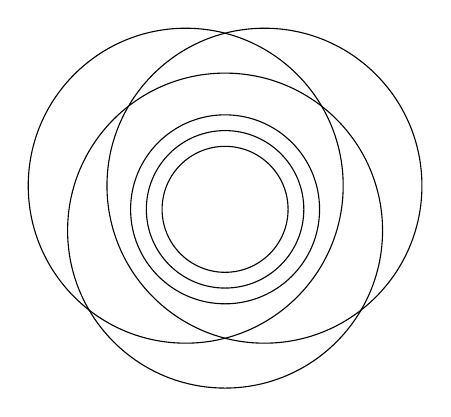
\begin{tikzpicture}
\draw (2,2) circle (2cm);
\draw (3,2) circle (2cm);
\draw (2.5,1.43) circle (2cm);
\draw (2.5,1.7) circle (1.2cm);
\draw (2.5,1.7) circle (1cm);
\draw (2.5,1.7) circle (0.8cm);
\end{tikzpicture}
\end{center}

Assume $B_\gamma\subset B_\beta\subset B_\alpha\subset U_i\cap U_j\cap U_k$, we need to check the following diagram commutes (the horizontal arrows are restriction maps in $\pzf_i,\pzf_j,\pzf_k$).
\begin{center}
\tiny
\begin{tikzcd}
\pzf_i(B_\alpha) \arrow[dd, "\phi_{ik}(B_\alpha)"'] \arrow[rd, "\phi_{ij}(B_\alpha)"] \arrow[rr] \arrow[rrrr, bend left] &  & \pzf_i(B_\beta) \arrow[dd, "\phi_{ik}(B_\beta)"'] \arrow[rd, "\phi_{ij}(B_\beta)"] \arrow[rr] &  & \pzf_i(B_\gamma) \arrow[dd, "\phi_{ik}(B_\gamma)"'] \arrow[rd, "\phi_{ij}(B_\gamma)"] &  \\
 & \pzf_j(B_\alpha) \arrow[ld, "\phi_{jk}(B_\alpha)"] \arrow[rr] \arrow[rrrr, bend left] &  & \pzf_j(B_\beta) \arrow[ld, "\phi_{jk}(B_\beta)"] \arrow[rr] &  & \pzf_j(B_\gamma) \arrow[ld, "\phi_{jk}(B_\gamma)"] \\
\pzf_k(B_\alpha) \arrow[rr] \arrow[rrrr, bend right] &  & \pzf_k(B_\beta) \arrow[rr] &  & \pzf_k(B_\gamma) & 
\end{tikzcd}
\end{center}
It commutes because of the cocycle condition.

Then for each equivalence class $[B_{i,\alpha}]\in \omega$, we can define $\pzf([B_{i,\alpha}])=\pzf_i(B_{i,\alpha})/\sim$, where the equivalence relation is just the isomorphism induced by $\phi_{ij}$. The restriction maps are also induced. 



It obviously forms a presheaf on the base $\omega$.

Base identity axiom:
For open sets $B$ in the base, there is $U_i$ containing it. $B=\cup_{i,\alpha\in A'_i}[B_{i,\alpha}]$. The base identity axiom holds because $\pzf_i$ is a sheaf on base of $U_i$. 

Base gluability holds similarly.

By previous theorem and exercises, there is a unique sheaf $\calf$ extending the sheaf on base $\pzf$.

Then it remains to check
$\calf|_{U_i}\cong\calf_i$. Notice that $\calf|_{U_i}([B_{i,\alpha}])=\calf([B_{i,\alpha}])=\pzf_i(B_{i,\alpha})=\calf_i(B_{i,\alpha})$. Recall the forgetful functor $\iota$ from category of sheaves to category of sheaves on a base, $\iota(\calf|_{U_i})\cong \pzf_i=\iota(\calf_i)$. Then $\calf|_{U_i}\cong \calf_i$ due to  exercise~\ref{chap2exr:equivalence_of_sheaves_on_base_and_sheaves}. (category of sheafs on $X$ is equivalent to the category of sheaves on a base of $X$)
\end{proof}


\begin{exr}\label{chap2exr:surjectivity_morphism_of_sheaves_checked_on_base}
Suppose a morphism of sheaves $\pzf\lrta\pzg$ on a base $\{B_i\}$ is surjective for all $B_i$ (i.e., $\pzf(B_i) \lrta \pzg(B_i)$ is surjective for all $i$). Show that the corresponding morphism of sheaves (not on the base) is surjective (or more precisely: an epimorphism).
\end{exr}
\begin{proof}
Recall~\ref{chap2:exr.surj_stalk_epimorphism_sheaf}, we can prove that surjective at the level of a base implies surjective at the level of stalks, which is true.
\end{proof}




\section{Sheaves of Abelian group, and $\calo_X$-modules, form Abelian categories}
\begin{exr}
Show that the stalk of the kernel is the kernel of the stalks: for all$ p \in  X$, there is a natural isomorphism
$$
(\ker(\calf\lrta \calg))_p\cong \ker (\calf_p\lrta \calg_p)
$$
\end{exr}
\begin{proof}
In exercise~\ref{chap2exr:kernel_sheaf}, we showed that the kernel of morphism of sheaves of abelian group is indeed a sheaf. The punchline is \textbf{filtered colimits preserve finite limits} (see \cite[p.~216]{mac1998categories}). There is no simple derivation using only the universal property. We have to prove it by hand. 

Consider the sheaf morphism $\phi:\calf\lrta \calg$.
Assume $[(f,U)]_p\in \ker(\calf\lrta\calg)_p$, where $(f,U)$ is a representative so that $f\in \ker (\phi(U))\in \calf(U)$.  Also $(\phi(U)f)_p=\phi_pf_p=0$, which means $f_p\in \ker(\phi_p)$. This gives a morphism from $\ker(\phi)_p$ to $\ker(\phi_p)$.

Then we construct the inverse. Given $f_p\in \ker(\phi_p)$, $\phi_pf_p=0$. Notice this means $\phi_p[(f';V)]=[(\phi(V)f';V)]=[(0;V)]$. Then there exists an open $W\ni p$ such that $\phi(W)f'|_W=0$. There is a representative of $f_p$ such that $f'|_W\in\ker \phi(W)$. This would mean $f'_p\in\ker(\phi)_p$, and we get a morphism from $\ker(\phi_p)$ to $\ker(\phi_p)$. Then it is routine to check that the two morphisms are mutually inverse.
\end{proof}

\begin{exr}
Show that the stalk of the cokernel is naturally isomorphic to the cokernel of the stalk.
\end{exr}
\begin{proof}
A cokernel in category of sheaves is the sheafification of cokernel in the category of presheaves. By Exercise~\ref{chap2:exr_shfification_iso_stalks}, sheafification induces isomorphism on stalks. then we only need to verify that the stalk of cokernel presheaves is isomorphic to cokernel of the stalks. But notice that 
$$
(\coker_{pre}(\phi))(U)=\coker(\phi(U)).
$$
Then because colimit commute with colimit we have 
$$
\coker_{pre}(\phi)_p\cong \coker(\phi_p).
$$
\end{proof}

\begin{exr}
Suppose $\phi:\calf\lrta \calg$ is a morphism of sheaves of Abelian groups. Show that the image sheaf $\im \phi$ is the sheafification of the image presheaf. Show that the stalk of the image is the image of the stalk.
\end{exr}
\begin{proof}
Recall the definition of images in Abelian category.

The image of a morphism $\phi : \calf \lrta \calg$ is defined as $\im(\phi) = \ker(\coker \phi)$ whenever it exists.

In the category of presheaves of Abelian groups, the kernel presheaves and cokernel presheaves do exists. And we already know $\coker(\phi)=\coker_{pre}(\phi)^{sh}$. We want to prove
$$
\ker_{pre}(\coker_{pre}(\phi))^{sh}=\ker(\coker_{pre}(\phi)^{sh})
$$
The punchline is \textbf{Sheafification commutes with finite limits} and ultimately, it relies on \textbf{filtered colimit commutes with finite limit}

\end{proof}
\textbf{As a consequnce, the exactness of a sequence of sheaves may be checked art the level of stalks.}
\begin{remark}
There is no direct simple minded proof based on abstract nonsense because it is not tautology. In the above exercise, sheafification commutes with finite limit in the category we care but its not tautology. If we want to have a try: We have two options, one is to check that $\ker_{pre}(\coker_{pre}(\phi))^{sh}$ satisfies the universal property of $\ker(\coker(\phi))$, another is to check that $\ker(\coker_{pre}(\phi)^{sh})$ satisfies the universal property of sheafification. For example, we try to prove that the sheafification has the universal property of being a kernel.
\begin{center}
\begin{tikzcd}
 & \calh \arrow[rrr, dashed] \arrow[ddd, dashed] &  &  & \calg \arrow[ddd, "\pi"'] \arrow[ldd, "\pi_{pre}"] \\
Z \arrow[rrrru] \arrow[rdd] \arrow[rr, dashed, "does\ not\ exists"'] &  & \calh_{pre} \arrow[ldd] \arrow[rru] \arrow[lu, "sh"] &  &  \\
 &  &  & \coker_{pre}(\phi) \arrow[rd, "sh"] &  \\
 & 0 \arrow[rrr] \arrow[rru] &  &  & \coker(\phi)
\end{tikzcd}
\end{center}
We denote $\calh_{pre}$ as $\ker(\coker_{pre}(\phi))$ and $\calh$ as its sheafification.
$Z\lrta \calg$ compose with $\calg\lrta \coker(\phi)$ to get $0$.
What we need is an arrow from $Z$ to $\calh$, but the universal property of sheafification at best can give us an arrow from $\calh$ to $Z$ and nothing else. We can neither construct the morphism from $Z$ to $\calh_{pre}$ because it would imply $\calh_{pre}=\calh$, which 
\end{remark}
\begin{exr}
Show that taking the stalk of a sheaf of abelian groups is an exact functor. More precsely, if $X$ is a toplogical space and $p\in X$ is a point, show that taking the stalk at $p$ defines an exact functor $Ab_X\lrta Ab$.
\end{exr}

\begin{exr}
Check that the exponential exact sequence is exact.
\end{exr}

\begin{exr}\label{chap2exr:left_exact_global_section}
Suppose $U\subset X$ is an open set, and $0\lrta \calf\lrta \calg\lrta \calh$ is an exact sequence of sheaves of abelian groups. Show that 
$$
0\lrta \calf(U)\lrta\calg(U)\lrta \calh(U)
$$
is exact. Show that the section functor need not be exact: show that if $0\lrta \calf\lrta \calg\lrta \calh\lrta 0$ is an exact sequence of sheaves of abelian groups, then
$$
0\lrta\calf(U)\lrta\calg(U)\lrta\calh(U)\lrta 0
$$
need not be exact.
\end{exr}

\begin{exr}
Suppose $\calf$ is a sheaf of abelian groups on a topological space $X$. Show that $\phom(\calf,\cot) $ is a left-exct covariant functor $Ab_X\lrta Ab_X$. Show that $\phom(\cdot,\calf)$ is a left excat contravaiant functor $Ab_X\lrta Ab_X$
\end{exr}

\begin{exr}
Show that given $(X,\calo_X)$ is a ringed space, then $\calo_X$-modules form an abelian category. 
\end{exr}
\begin{exr}\label{chap2exr:sheaf_section_functor_left_excact}
\ \begin{enumerate}[label=(\alph*)]
\item Suppose $\calo_X$ is a sheaf of rings on $X$. Define (categorically) what we should mean by \textbf{ tensor product of two $\calo_X$-modules.} Given an explicit construction, and show that it satisfies your categorical definition.
\item Show that the tensor product of stlks is the stalk of the tensor product. (colimits commute with tensor products)
\end{enumerate}
\end{exr}
\section{The inverse image sheaf}
\begin{exr}
Show that the map
$$
\pi^{-1}_{pre}\calg(U)=\colim_{}V\supset \pi(U)\calg(V).
$$
 defines a presheaf on $X$. Show that it needn’t form a sheaf. 
\end{exr}

\begin{exr}\label{chap2exr:adjoint_inverse_image_direct_image}
If $\pi:X\lrta Y$ is a continuous map, and $\calf$ is a shef on $X$ and $\calg$ is a sheaf on $Y$. describe a bijection 
$$
\mor(\pi^{-1}\calg,\calf)\llrta\mor(\calg,\pi_*\calf).
$$
\end{exr}

\begin{exr}
Show that the stalks of $\pi^{-1}\calg$ are the same as the stalks of $\calg$. More precisely, if $\pi(p)=q$, describe a natural isomorphism $\calg_q\lrta (\pi^{-1}\calg)_p$.
\end{exr}

\begin{exr}
If $U$ is an open subset of $Y$, $i:U\lrta Y$ is the inclusion, and $\calg$ is a sheaf on $Y$, show that $i^{-1}Y$ is naturally isomorphic to $\calg|_U$
\end{exr}